\documentclass[12pt]{article}
\usepackage[utf8]{inputenc}
\usepackage[UTF8]{ctex}
\usepackage{biblatex}
\usepackage{amssymb}
\usepackage{latexsym}
\usepackage{amsmath}
\usepackage{geometry}
\usepackage{graphicx}
\usepackage{listings}
\lstset{
    basicstyle          =   \sffamily,          
    keywordstyle        =   \bfseries,        
    commentstyle        =   \rmfamily\itshape,  
    stringstyle         =   \ttfamily,  
    flexiblecolumns,             个
    numbers             =   left,   
    showspaces          =   false,  
    numberstyle         =   \zihao{-5}\ttfamily,    
    showstringspaces    =   false,
    captionpos          =   t,      
    frame               =   lrtb,   
}
\lstdefinestyle{Python}{
    language        =   Python, 
    basicstyle      =   \zihao{-5}\ttfamily,
    numberstyle     =   \zihao{-5}\ttfamily,
    keywordstyle    =   \color{blue},
    keywordstyle    =   [2] \color{teal},
    stringstyle     =   \color{magenta},
    commentstyle    =   \color{red}\ttfamily,
    breaklines      =   true,   
    columns         =   fixed,  
    basewidth       =   0.5em,
}
\addbibresource{bib.bib}
\setlength{\parindent}{0em}
\bibliography{bib}
\geometry{a4paper,scale=0.8}

\title{光子计数研究报告}
\author{郭远洋,章于,张可}
\date{2021年5月25日}
\linespread{1.5}
\graphicspath{{Images/}}
\begin{document}

\maketitle

\section{课题背景}
\textbf{光子计数器与光子计数过程}

光子计数器是一种可以测量光子级别微弱能量的无限光通信信号检测设备。它可以将微弱光信号能量转化为数值形式的光子数,便于后续的数字信号处理。但是,由于光电量子效应的存在,光子计数器并不能完美得到所接收到的光子数。在一个有限长的符号时间内,光子计数过程宏观表现为泊松分布。这意味着光子计数器引入了新的噪声,称为泊松散弹噪声。

离散时间泊松信道(Discrete-Time Poisson,DTP)是通用地描述泊松散弹噪声影响下光子计数过程的数学模型。需要注意的是,DTP研究的是光子计数器内部散弹噪声,与传统AWGN信道有很大的区别。输出Y是满足以信道输入为参数的泊松分布,即
$$Pr(Y=y|\Lambda=\lambda)=\frac{\lambda^y}{y!}e^{-\lambda} \eqno{(1)}$$
对于完美的光子计数接收端,其可以无误差的检测每个光子以及它的到达时间。然而,完美的光子计数接收端难以实现,我们更关注于非完美的接收端。当光子到达时,探测器产生具有特定宽度的脉冲,当两个光子的到达时间间隔比脉冲宽度短,则会造成两个脉冲合并到一起。两个脉冲合并到一起时的最大不可区分的光子到达时间间隔被称为死时间。
非理想光子计数器的计数值服从二项分布:
$$Pr(Y=y | \Lambda=\lambda)=C^{y}_{N}\left(1-e^-\frac{\lambda}{N}\right)^y\left(e^-\frac{\lambda}{N}\right)^{N-y} \eqno{(2)}$$

\section{课题内容}
\subsection{求解Q-PAM调制SISO互信息}

在Q进制脉冲振幅(Q-PAM)调制下,
$$\Lambda = X\cdot\frac{n_s}{Q}+n_b \eqno{(3)}$$
其中$n_b$为激光器最大发射光子数,$X$是调制后的Q进制信息,则$X\cdot\frac{n_s}{Q}$为激光器在发射信息为$X$时发射的光子数。$n_b$是恒定的背景光噪声光子数。假定发射信息是等概的,即:
$$Pr(X=x,x=1,2,...,Q)=\frac{1}{Q} \eqno{(4)}$$
将(4)带入(2)可得Q-PAM调制下SISO的输出服从:
$$Pr(Y=y|X=x)=C^{y}_{N}\left[1-exp\left(-\frac{x\cdot\frac{n_s}{Q}+n_b}{N}\right)\right]^y\cdot\left[exp\left(-\frac{x\cdot\frac{n_s}{Q}+n_b}{N}\right)\right]^{N-y} \eqno{(5)}$$
求互信息$I(X;Y)$。

\subsection{求解OOK调制SIMO互信息}

在开关键控(OOK)调制下,第n路输出为:$$\Lambda_n=X\cdot h_s\cdot n_s + n_b \eqno{(6)}$$
其中$n_s$为激光器打开时的发射光子数,$X$是调制后的二进制信息,$h_n$为SIMO系数。$n_b$是恒定的背景光噪声光子数。假设发射信息是等概的。
将(6)带入(2)可得OOK调制下DTP-SIMO信道的输出服从:$$Pr(Y_n=y_n|X=x)=C^{y_n}_{N}\left[1-exp\left(-\frac{x\cdot h_n\cdot n_s+n_b}{N}\right)\right]^{y_n} \left[exp\left(-\frac{x\cdot h_n\cdot n_s+n_b}{N}\right)\right]^{N-y_n} \eqno{(7)}$$
求和速率$I(X;Y)=\sum\limits_{n=1}^{N}I(X;Y_n)$。

\newpage
\subsection{求解OOK调制MIMO互信息}

在开关键控(OOK)调制下,m路输入n路输出:
$$\Lambda_{m,n}=X_m\cdot h_{m,n}\cdot n_{sm} + n_{bm} \eqno{(8)}$$
其中$n_{sm}$为第m路激光器打开时的发射光子数, $X_m$是调制后的二进制信息, 为MIMO系数。 $n_{bm}$是平均到每路的恒定的背景光噪声光子数。若定义总背景光噪声光子数为$n_b$,显然$\displaystyle n_{bm}=\frac{n_b}{M}$。假定发射信息是等概的,即:
$$Pr(X_m=0,∀m=1,2,...,M)=Pr(X_m=1,∀m=1,2,...,M)=\frac{1}{2} \eqno{(9)}$$
将(8)带入(2)可得第$l$时隙Q-PAM调制下第n路DTP-MIMO信道的输出服从:
$$Pr(Y_n=y_n|X_m=x_m,m=1,2,...,M)=$$
$$C^{y_n}_{N}\left[1-exp\left(-\frac{\sum\limits_{m=1}^{M}h_{m,n}x_mn_{sm}+n_b}{N}\right)\right]^{y_n} \left[exp\left(-\frac{\sum\limits_{m=1}^{M}h_{m,n}x_mn_{sm}+n_b}{N}\right)\right]^{N-y_n} \eqno{(10)}$$
求M=2, N=4时的和速率$\sum\limits_{n=2}^{4}I_n(X_1,X_2;Y_n)$。
其中$I_n(X_1,X_2;Y_n)$为第n路的无条件互信息。

\subsection{求解大背景光下OOK调制DTP-MIMO互信息}

当$n_b$较大时,由于泊松分布的特性,可近似为高斯分布。近似后概率密度函数为:
$$f(Y_n=y_n|X_m=x_m,m=1,2,...,M)=\frac{exp\left\{-\frac{\left[y_n-\left(\sum\limits_{m=1}^Mh_{m,n}x_mn_{sm}+n_b\right)\right]^2}{2\left(\sum\limits_{m=1}^Mh_{m,n}x_mn_{sm}+n_b\right)}\right\}}{\sqrt{2\pi\left(\sum\limits_{m=1}^Mh_{m,n}x_mn_{sm}+n_b\right)}} \eqno{(11)}$$
求M=2,N=4时的和速率$\sum\limits_{n=1}^4I\left(X_1,X_2;Y_n\right)$。

\section{课题推导过程}
\subsection{求解Q-PAM调制SISO互信息}
定义$\Lambda=X·\frac{n_s}{Q}+n_b,t_i=x_i·\frac{n_s}{Q}+n_b,t_Q=n_s+n_b,P_{t_i}(y)=Pr(y|x_i)=C^{y}_{N}\left(1-e^{-\frac{t_i}{N}}\right)^y\left(e^{-\frac{t_i}{N}}\right)^{N-y}$:
那么有:
\begin{equation*}
  \begin{aligned}
    I(X;Y) &= H(Y)-H(Y|X) \\
      &= -\sum\limits_{j=0}^{N}Pr(y_i)log_2Pr(y_j)+\sum_{ij}P_{t_i}(y_j)P(x_i)log_2P_{t_i}(y_j) 
  \end{aligned}
\end{equation*}
$X$的各取值等概,所以$P(x_i)=\frac{1}{Q}$。
\begin{equation*}
  \begin{aligned}
    I(X;Y) &= -\sum\limits_{j=0}^{N}\left\{\left[\sum\limits_{i=0}^Q\frac{1}{Q}P_{t_i}(y_j)\right]log_2\left[\sum\limits_{i=1}^Q\frac{1}{Q}P_{t_i}(y_j)\right]\right\}+\frac{1}{Q}\sum\limits_{j=0}^N\sum\limits_{i=0}^{Q}\left[P_{t_i}(y_j)log_2P_{t_i}(y_j)\right]  \\
      &= -\frac{1}{Q}\sum\limits_{j=0}^{N}\left\{\left[\sum\limits_{i=0}^QP_{t_i}(y_j)\right]log_2\left[\frac{1}{Q}\sum\limits_{i=1}^QP_{t_i}(y_j)\right]\right\}+\frac{1}{Q}\sum\limits_{j=0}^N\sum\limits_{i=0}^{Q}\left[P_{t_i}(y_j)log_2P_{t_i}(y_j)\right]  
      
  \end{aligned}
\end{equation*}
将上式中$\sum\limits_{j=0}^{N}y_j$均改为$\sum\limits_{y=0}^{N}y$后:
\begin{equation*}
  \begin{aligned}
    I(X;Y) =& -\frac{1}{Q}\sum\limits_{y=0}^{N}\left\{\left[\sum\limits_{i=0}^QP_{t_i}(y)\right]\left[log_2\left(\sum\limits_{i=1}^Q\frac{P_{t_i}(y)}{P_{t_Q}(y)}\right)-log_2Q\right]\right\} + \frac{1}{Q}\sum\limits_{y=0}^{N}\left\{\sum\limits_{i=0}^{Q-1}\left[P_{t_i}(y)log_2\frac{P_{t_i}(y)}{P_{t_Q}(y)}\right]\right\} \\
    =& -\frac{1}{Q}\sum\limits_{y=0}^{N}\left\{\left[\sum\limits_{i=0}^QP_{t_i}(y)\right]\left[log_2\left(\sum\limits_{i=1}^Q\frac{P_{t_i}(y)}{P_{t_Q}(y)}\right)\right]\right\} + \frac{1}{Q}\left[\sum\limits_{y=0}^{N}\sum\limits_{i=0}^{Q-1}P_{t_i}(y)\right]·log_2Q \\
    &+ \frac{1}{Q}\sum\limits_{y=0}^{N}\left\{\sum\limits_{i=0}^{Q-1}\left[P_{t_i}(y)log_2\frac{P_{t_i}(y)}{P_{t_Q}(y)}\right]\right\} \\
    =& I_1 + log_2Q + I_2
  \end{aligned}
\end{equation*}
$I_1=-\frac{1}{Q}\sum\limits_{y=0}^{N}\left\{\left[\sum\limits_{i=1}^QP_{t_i}(y)\right]\left[log_2\left(\sum\limits_{i=1}^Q\frac{P_{t_i}(y)}{P_{t_Q}(y)}\right)\right]\right\}$\par
\par\par 利用Taylor展开:$ln(1+x)\approx x$得到:
$$log_2\left(\sum\limits_{i=1}^Q\frac{P_{t_i}}{P_{t_Q}}\right)=log_2e·ln\left(\sum\limits_{i=1}^{Q-1}\frac{P_{t_i}}{P_{t_Q}}+1\right)\approx log_2e\left(\sum\limits_{i=1}^{Q-1}\frac{P_{t_i}}{P_{t_Q}}\right)$$
\newpage
所以:\par
\begin{equation*}
  \begin{aligned}
    I_1 &= -\frac{1}{Q}log_2e\sum\limits_{y=0}^{N}\left[\left(\sum\limits_{i=1}^QP_{t_i}(y)\right)\left(\sum\limits_{i=1}^{Q-1}\frac{P_{t_i}(y)}{P_{t_Q}(y)}\right)\right] \\
    &= -\frac{1}{Q}log_2e\sum\limits_{y=0}^{N}\left[\left(\sum\limits_{i=1}^{Q-1}P_{t_i}(y)\right)\left(\sum\limits_{i=1}^{Q-1}\frac{P_{t_i}(y)}{P_{t_Q}(y)}\right)+\sum\limits_{i=1}^{Q-1}P_{t_i}(y)\right] \\
    &=  -\frac{1}{Q}log_2e\sum\limits_{y=0}^{N}\left[\left(\sum\limits_{i=1}^{Q-1}P_{t_i}(y)\right)\left(\sum\limits_{i=1}^{Q-1}\frac{P_{t_i}(y)}{P_{t_Q}(y)}\right)\right]-\frac{Q-1}{Q}log_2e
  \end{aligned}
\end{equation*}
带入$P_{t_i}(y)=Pr(y|x_i)=C^{y}_{N}\left(1-e^{-\frac{t_i}{N}}\right)^y\left(e^{-\frac{t_i}{N}}\right)^{N-y}$:\par
\begin{equation*}
    \sum\limits_{y=0}^N\left[P_{t_i}(y)\frac{P_{t_j(y)}}{{P_{t_Q}(y)}}\right] =\sum\limits_{y=0}^NC_N^y\left[\frac{\left(1-e^{-\frac{t_i}{N}}\right)\left(1-e^{-\frac{t_j}{N}}\right)}{1-e^{-\frac{t_Q}{N}}}\right]^y·\left(\frac{e^{-\frac{t_i}{N}}·\frac{e^{-\frac{t_j}{N}}}}{e^{-\frac{t_Q}{N}}}\right)^{N-y}
\end{equation*}
利用$(a+b)^N=\sum\limits_{y=0}^NC_N^ya^yb^{N-y}$,并将上一般交叉项代入原$I_1$中,即:\par
\begin{equation*}
  \begin{aligned}
    I_1 &= -\frac{Q-1}{Q}log_2e-\frac{1}{Q}log_2e·\sum_{i,j=1,2,···,Q-1}\left[\frac{\left(1-e^{-\frac{t_i}{N}}\right)\left(1-e^{-\frac{t_j}{N}}\right)}{1-e^{-\frac{t_Q}{N}}}+e^{\frac{t_Q-t_j-t_i}{N}}\right]^N \\
    I_2 &= \frac{1}{Q}\sum\limits_{y=0}^N\left\{\sum\limits_{i=0}^{Q-1}\left[P_{t_i}(y)log_2\frac{P_{t_i}(y)}{P_{t_Q}(y)}\right]\right\} \\
    &= \frac{1}{Q}\sum\limits_{y=0}^N\left\{\sum\limits_{i=1}^{Q-1}\left[P_{t_i}(y)log_2\frac{C_N^y\left(1-e^{-\frac{t_i}{N}}\right)^y\left(e^{-\frac{t_i}{N}}\right)^{N-y}}{C_N^y\left(1-e^{-\frac{t_Q}{N}}\right)^y\left(e^{-\frac{t_Q}{N}}\right)^{N-y}}\right]\right\} \\
    &= \frac{1}{Q}\sum\limits_{y=0}^N\left\{\sum\limits_{i=1}^{Q-1}\left[yP_{t_i}(y)log_2\left(\frac{1-e^{-\frac{t_i}{N}}}{1-e^{-\frac{t_Q}{N}}}\right)+(N-y)P_{t_i}(y)log_2\left(\frac{e^{-\frac{t_i}{N}}}{e^{-\frac{t_Q}{N}}}\right)\right]\right\}
  \end{aligned}
\end{equation*}
交换求和次序:\par
\begin{equation*}
  \begin{aligned}
    I_2 &= \frac{1}{Q}\sum\limits_{i=1}^{Q-1}\left\{\sum\limits_{y=0}^N\left[yP_{t_i}(y)log_2\left(\frac{1-e^{-\frac{t_i}{N}}}{1-e^{-\frac{t_Q}{N}}}\right)\right] - \sum\limits_{y=0}^N\left[yP_{t_i}(y)log_2\left(\frac{e^{-\frac{t_i}{N}}}{e^{-\frac{t_Q}{N}}}\right)\right] +N\sum\limits_{y=0}^NP_{t_i}(y)log_2\left(\frac{e^{-\frac{t_i}{N}}}{e^{-\frac{t_Q}{N}}}\right) \right\}
  \end{aligned}
\end{equation*}
利用$E(y)=\sum\limits_{y=0}^NyP_{t_i}(y)$,二项分布$E(y)=N(1-P_i)$,其中$P_i=e^{-\frac{t_i}{N}}$:\par
\begin{equation*}
  \begin{aligned}
    I_2 &= \frac{1}{Q}\sum\limits_{i=1}^{Q-1}\left[N(1-P_i)·log_2\left(\frac{1-e^{-\frac{t_i}{N}}}{1-e^{-\frac{t_Q}{N}}}\right)\right]-\frac{1}{Q}\sum\limits_{i=1}^{Q-1}\left[N(1-P_i)·log_2\left(\frac{e^{-\frac{t_i}{N}}}{e^{-\frac{t_Q}{N}}}\right)\right]+\frac{N}{Q}\sum\limits_{i=1}^{Q-1}log_2\left(\frac{e^{-\frac{t_i}{N}}}{e^{-\frac{t_Q}{N}}}\right)
  \end{aligned}
\end{equation*}
将$I_1,I_2$带入$I(X;Y)$:\par
\begin{equation*}
  \begin{aligned}
    I(X;Y) &= I_1+I_2+log_2Q,\ let\ e^{-\frac{t_i}{N}}=P_i :\\
    =& log_2Q+\frac{1}{Q}\sum\limits_{i=1}^{Q-1}\left(N(1-P_i)·log_2\frac{1-P_1}{1-P_Q}-N(1-P_i)·log_2\frac{P_1}{P_Q}+Nlog_2\frac{P_i}{P_Q}\right)-\frac{Q-1}{Q}log_2e \\
    &- \frac{1}{Q}log_2e\sum\limits_{i,j=1,2,···,Q-1}\left[\frac{(1-P_i)(1-P_j)}{1-P_Q}+\frac{P_iP_j}{P_Q}\right]^N \\
    =& log_2Q-\frac{Q-1}{Q}log_2e+\frac{N}{Q}\sum\limits_{i=1}^{Q-1}\left[log_2\left(\frac{1-P_i}{1-P_Q}·\frac{P_Q}{P_i}\right)^{1-P_i}·\frac{P_i}{P_Q}\right]\\
    &- \frac{1}{Q}log_2e\sum\limits_{i,j=1,2,···,Q-1}\left[\frac{(1-P_i)(1-P_j)}{1-P_Q}+\frac{P_iP_j}{P_Q}\right]^N
  \end{aligned}
\end{equation*}
以上即为最终结果。
但是,在$ln(1+x)~x$这一步存在一定误差,故我们使用另一个用来直接拟合$lnx$的函数$f(x)=\frac{n}{2}\left(x^{\frac{1}{n}}-x^{-\frac{1}{n}}\right)$,当$n$非常大时,拟合的效果很好。
受限于精力与算力,我们取$n=2$的情况计算,即$lnx~x^{\frac{1}{2}}-x^{-\frac{1}{2}}$,计算如下:
\begin{equation*}
  \begin{aligned}
    I_1 &= -\frac{1}{Q}\sum\limits_{y=0}^{N}\left\{\left[\sum\limits_{i=1}^QP_{t_i}(y)\right]\left[log_2\left(\sum\limits_{i=1}^Q\frac{P_{t_i}(y)}{P_{t_Q}(y)}\right)\right]\right\} \\
    &= -\frac{1}{Q}log_2e\sum\limits_{y=0}^{N}\left\{\left[\sum\limits_{i=1}^QP_{t_i}(y)\right]\left[\left(\sum\limits_{i=1}^Q\frac{P_{t_i}(y)}{P_{t_Q}(y)}\right)^{\frac{1}{2}}-\left(\sum\limits_{i=1}^Q\frac{P_{t_i}(y)}{P_{t_Q}(y)}\right)^{-\frac{1}{2}}\right]\right\} \\
    &= -\frac{1}{Q}log_2e\sum\limits_{y=0}^{N}\left[P_{t_Q}(y)\sum\limits_{i=1}^{Q-1}\frac{P_{t_i}(y)}{P_{t_Q}(y)}·\left(\sum\limits_{i=1}^{Q-1}\frac{P_{t_i}(y)}{P_{t_Q}(y)}+1\right)^{\frac{1}{2}}\right]
  \end{aligned}
\end{equation*}
令$a_i=\frac{P_{t_i}}{P_{t_Q}}$带入$I_1$中:
$$I_1=-\frac{1}{Q}log_2e\sum\limits_{y=0}^{N}\left[P_{t_Q}(y)\sum\limits_{i=1}^{Q-1}a_i·\left(\sum\limits_{i=1}^{Q-1}a_i+1\right)^{\frac{1}{2}}\right]$$
利用无穷级数将$\frac{1}{2}$幂次方展开:
\begin{equation*}
  \begin{aligned}
    I_1 &= -\frac{1}{Q}log_2e\sum\limits_{y=0}^{N}\left[P_{t_Q}(y)\sum\limits_{i=1}^{Q-1}a_i·\sum\limits_{k=0}^{\infty}\left(^{\frac{1}{2}}_k\right)\left(\sum\limits_{i=1}^{Q-1}a_i\right)^{k}\right] \\
    &= -\frac{1}{Q}log_2e\sum\limits_{y=0}^{N}\left[P_{t_Q}(y)\sum\limits_{k=0}^{\infty}\left(^{\frac{1}{2}}_k\right)\sum\limits_{k_1+k_2+···+k_{Q-1}=k+1}a_1^{k_1}a_2^{k_2}···a_{Q-1}k_{Q-1}\frac{(k+1)!}{k_1!k_2!···k_{Q-1}!}\right] \\
    =& -\frac{1}{Q}log_2e\sum\limits_{k=0}^{\infty}\left(^{1/2}_k\right)\sum\limits_{\sum_{i=1}^{Q-1}k_i=k+1}\left\{\frac{(k+1)!}{\prod_{i=1}^{Q-1}k_i!}\sum\limits_{y=0}^NC_N^y\left[\prod_{i=0}^{Q-1}\left(\frac{1-e^{-\frac{t_i}{N}}}{1-e^{-\frac{t_Q}{N}}}\right)^{k_i}·\left(1-e^{-\frac{t_Q}{N}}\right)\right]^y\right\} \\
    &·\left[\prod_{i=1}^{Q-1}e^{\left(\frac{(Q-i)n_s}{QN}\right)^{k_i}}e^{-\frac{t_Q}{N}}\right]^{N-y}
  \end{aligned}
\end{equation*}
利用二项式定理$\sum_{y=0}^NC_N^ya^yb^{N-y}=(a+b)^N$带入$I_1$中,令$P_i=e^{\frac{t_i}{N}}$:
$$I_1=-\frac{1}{Q}log_2e\sum\limits_{k=0}^\infty\left(^{1/2}_k\right)\sum\limits_{\sum_{i=1}^{Q-1}k_i=k+1}\left\{\frac{(k+1)!}{\prod_{i=1}^{Q-1}k_i!}\left[(1-P_Q)\prod_{i=1}^{Q-1}\left(\frac{1-P_i}{1-P_Q}\right)^{k_i}+P_Q\prod_{i=1}^{Q-1}e^{\left(\frac{Q-i}{NQ}n_s\right)^{k_i}}\right]^N\right\}$$
$I(X;Y)=I_1+I_2+log_2Q$
下面尝试利用n计算$I(X;Y)$,即$ln(x)\approx\frac{m}{2}\left(x^{\frac{1}{m}}-x^{-\frac{1}{m}}\right)$:
\begin{equation*}
  \begin{aligned}
    I_1 &= -\frac{1}{Q}\sum\limits_{y=0}^N\left\{\left[\sum\limits_{i=1}^QP_{t_i}(y)\right]\left[log_2\left(\sum\limits_{i=1}^Q\frac{P_{t_i}(y)}{P_{t_Q}(y)}\right)\right]\right\} \\
    &=-\frac{m}{2Q}log_2e\sum\limits_{y=0}^N\left\{\left[\sum\limits_{i=1}^QP_{t_i}(y)\right]\left[\left(\sum\limits_{i=1}^Q\frac{P_{t_i}(y)}{P_{t_Q}(y)}\right)^{\frac{1}{m}}-\left(\sum\limits_{i=1}^Q\frac{P_{t_i}(y)}{P_{t_Q}(y)}\right)^{-\frac{1}{m}}\right]\right\} \\
    &=-\frac{m}{2Q}log_2e\sum\limits_{y=0}^NP_{t_Q}(y)\left[\left(\sum\limits_{i=1}^Q\frac{P_{t_i}(y)}{P_{t_Q}(y)}\right)^{1+\frac{1}{m}}-\left(\sum\limits_{i=1}^Q\frac{P_{t_i}(y)}{P_{t_Q}(y)}\right)^{1-\frac{1}{m}}\right]
  \end{aligned}
\end{equation*}
将$a_i=\frac{P_{t_i}(y)}{P_{t_Q}(y)}$代入:
\begin{equation*}
  \begin{aligned}
    I_1 =& -\frac{m}{2Q}log_2e\sum\limits_{y=0}^NP_{t_Q}(y)\left\{\sum\limits_{k=0}^\infty\left(^{1+1/m}_k\right)\sum\limits_{k_1+k_2+···+k_{Q-1}=k}a_1^{k_1}···a_{Q-1}^{k_{Q-1}}\frac{k!}{k_1!k_2!···k_{Q-1}!} \\ 
    &-\sum\limits_{g=0}^\infty\left(^{1+1/m}_g\right)\sum\limits_{\sum_{i=1}^{Q-1}g_i=g}a_1^{g_1}···a_{Q-1}^{g_{Q-1}}\frac{g!}{g_1!g_2!···g_{Q-1}!}\right\} \\
    =& -\frac{m}{2Q}log_2e\left\{\sum\limits_{k=0}^\infty\left(^{1+1/m}_k\right)\sum\limits_{\sum_{i=1}^{Q-1}k_i=k}\frac{k!}{\prod_{i=1}^{Q-1}k_i!}\left[\prod_{i=1}^{Q-1}\left(\frac{1-e^{-\frac{t_i}{N}}}{1-e^{-\frac{t_Q}{N}}}\right)^{k_i}·\left(1-e^{-\frac{t_Q}{N}}\right)+\prod_{i=1}^{Q-1}e^{\frac{k_i(t_Q-t_i)-t_Q}{N}}\right]^N \\
    &-\sum\limits_{g=0}^\infty\left(^{1+1/m}_g\right)\sum\limits_{\sum_{i=1}^{Q-1}g_i=g}\frac{g!}{\prod_{i=1}^{Q-1}g_i!}\left[\prod_{i=1}^{Q-1}\left(\frac{1-e^{-\frac{t_i}{N}}}{1-e^{-\frac{t_Q}{N}}}\right)^{g_i}·\left(1-e^{-\frac{t_Q}{N}}\right)+\prod_{i=1}^{Q-1}e^{\frac{g_i(t_Q-t_i)-t_Q}{N}}\right]^N\right\}
  \end{aligned}
\end{equation*}
使用以下代码绘图(具体的代码分析和仿真分析见仿真报告):
\lstinputlisting[
    style       =   Python,
    caption     =   {\bf Matlab Program},
    label       =   {ff.py}
]{Code_of_Q1.txt}
\newpage
\begin{figure}[htbp]
\centering
\begin{minipage}[t]{0.48\textwidth}
\centering
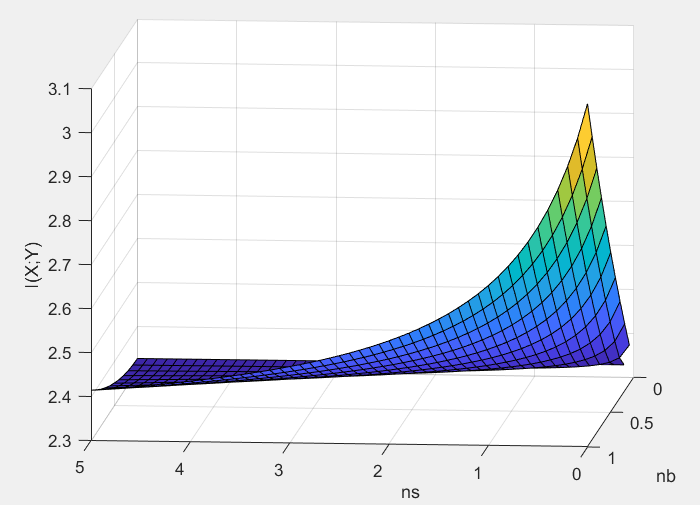
\includegraphics[width=7.5cm]{Image_of_Q1RE.png}
\end{minipage}
\begin{minipage}[t]{0.48\textwidth}
\centering
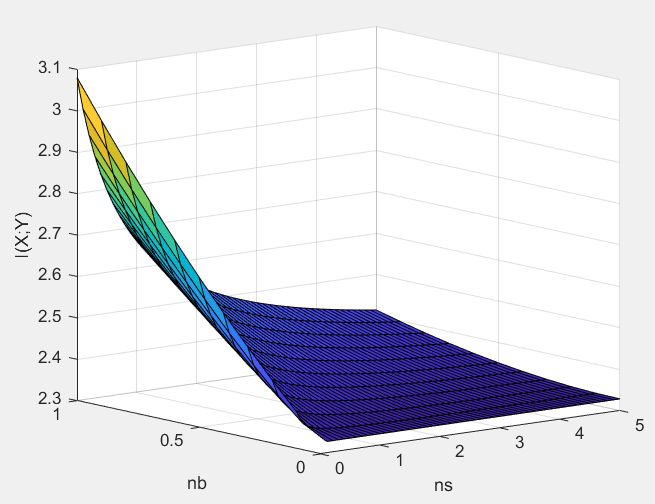
\includegraphics[width=7cm]{Image_of_Q2RE.png}
\end{minipage}
\end{figure}

\subsection{求解OOK调制SIMO互信息}
定义:\par$\Lambda_n=X·h_n·n_s+n_b$\par$t_i=x_ih_nn_s+n_b$\par$P_r(Y_n=y_n|X=x_i)=C_N^{y_n}\left[1-exp\left(-\frac{t_i}{N}\right)\right]^{y_n}·\left[exp\left(-\frac{t_i}{N}\right)\right]^{N-y_n}$\par$I(X;Y)=H(Y_n)-H(Y_n|X)$\par$t_Q=n_b$,$t_1=h_nn_s+n_b$\par
那么,可以得到:
\begin{equation*}
    \begin{aligned}
      H(Y_n)=&-\sum\limits_{y_n=0}^N\left[\frac{1}{2}P_r(Y_n=y_n|x=0)+\frac{1}{2}P_r(Y_n=y_n|x=1)\right] \\
      &·log_2\left[\frac{1}{2}P_r(Y_n=y_n|x=0)+\frac{1}{2}P_r(Y_n=y_n|x=1)\right]
    \end{aligned}
\end{equation*}
\begin{equation*}
    \begin{aligned}
      H(Y_n|X)=&-\frac{1}{2}\sum\limits_{y_n=0}^NP_r(Y_n=y_n|x=0)log_2[P_r(Y_n=y_n|x=0)] \\
      &-\frac{1}{2}\sum\limits_{y_n=0}^NP_r(Y_n=y_n|x=1)log_2[P_r(Y_n=y_n|x=1)]
    \end{aligned}
\end{equation*}
\begin{equation*}
    \begin{aligned}
      \Rightarrow H(Y_n)&=-\sum\limits_{y_n=0}^N\left[\frac{1}{2}P_r(Y_n=y_n|x=0)+\frac{1}{2}P_r(Y_n=y_n|x=1)\right]log_2\left[\frac{1}{2}\frac{P_r(Y_n=y_n|x=0)}{P_r(Y_n=y_n|x=1)}+\frac{1}{2}\right]
    \end{aligned}
\end{equation*}
\begin{equation*}
    \begin{aligned}
       H(Y_n|x)=&-\frac{1}{2}\sum\limits_{y_n=0}^N\left[\frac{1}{2}P_r(Y_n=y_n|x=0)+\frac{1}{2}P_r(Y_n=y_n|x=1)\right]log_2\frac{P_r(Y_n=y_n|x=0)}{P_r(Y_n=y_n|x=1)}\\
       &-\frac{1}{2}\sum\limits_{y_n=0}^N\left[\frac{1}{2}P_r(Y_n=y_n|x=0)+\frac{1}{2}P_r(Y_n=y_n|x=1)\right]log_2P_r(Y_n=y_n|x=1)
    \end{aligned}
\end{equation*}
发现$H(Y_n)$和$H(Y_n|X)$的第二项加式相同,则:
\begin{equation*}
    \begin{aligned}
       I(X;Y_n)=&H(Y_n)-H(Y_n|X) \\
       =&-\sum\limits_{y_n=0}^N\left[\frac{1}{2}P_r(Y_n=y_n|x=0)+\frac{1}{2}P_r(Y_n=y_n|x=1)\right]log_2\left[\frac{1}{2}\frac{P_r(Y_n=y_n|x=0)}{P_r(Y_n=y_n|x=1)}+\frac{1}{2}\right] \\
       &+\frac{1}{2}\sum\limits_{y_n=0}^NP_r(Y_n=y_n|x=0)log_2\frac{P_r(Y_n=y_n|x=0)}{P_r(Y_n=y_n|x=1)} \\
       =&1-\sum\limits_{y_n=0}^N\left[\frac{1}{2}P_r(Y_n=y_n|x=0)+\frac{1}{2}P_r(Y_n=y_n|x=1)\right]log_2\left[\frac{P_r(Y_n=y_n|x=0)}{P_r(Y_n=y_n|x=1)}+1\right] \\
       &+ \frac{1}{2}\sum\limits_{y_n=0}^NP_r(Y_n=y_n|x=0)log_2\frac{P_r(Y_n=y_n|x=0)}{P_r(Y_n=y_n|x=1)}
    \end{aligned}
\end{equation*}
有:
\begin{equation*}
    \begin{aligned}
       P_r(Y_n=y_n|x=0)=&C_N^{y_n}\left[1-exp\left(-\frac{n_b}{N}\right)\right]^{y_n}\left[exp\left(-\frac{n_b}{N}\right)\right]^{N-y_n}=C_N^{y_n}·\left[1-e^{-\frac{t_0}{N}}\right]^{y_n}·e^{-\frac{t_0}{N}(N-y_n)} \\
       P_r(Y_n=y_n|x=1)=&C_N^{y_n}\left[1-exp\left(-\frac{h_n·n_s+n_b}{N}\right)\right]^{y_n}\left[exp\left(-\frac{h_n·n_s+n_b}{N}\right)\right]^{N-y_n} \\
       =&C_N^{y_n}·\left[1-e^{-\frac{t_1}{N}}\right]^{y_n}·e^{-\frac{t_1}{N}(N-y_n)} \\
       \frac{P_r(Y_n=y_n|x=0)}{P_r(Y_n=y_n|x=1)}&=\left(\frac{1-e^{-\frac{t_0}{N}}}{1-e^{-\frac{t_1}{N}}}\right)^{y_n}·e^{\frac{t_1-t_0}{N}(N-y_n)} \\
       I(X;y_n)=&1-\sum\limits_{y_n=0}^NC_N^{y_n}·\frac{1}{2}\left\{\left[1-e^{-\frac{t_0}{N}}\right]^{y_n}·e^{-\frac{t_0}{N}(N-y_n)}+\left[1-e^{-\frac{t_1}{N}}\right]^{y_n}·e^{-\frac{t_1}{N}(N-y_n)}\right\} \\
       &·log_2\left\{\left[\frac{1-e^{-\frac{t_0}{N}}}{1-e^{-\frac{t_1}{N}}}\right]^{y_n}·e^{[\frac{t_1-t_0}{N}(N-y_n)]}+1\right\} \\
       &+\frac{1}{2}\sum\limits_{y_n=0}^NC_N^{y_n}\left[1-e^{-\frac{t_0}{N}}\right]^{y_n}e^{-\frac{t_0}{N}(N-y_n)}log_2\left\{\left[\frac{1-e^{-\frac{t_0}{N}}}{1-e^{-\frac{t_1}{N}}}\right]^{y_n}e^{[\frac{t_1-t_0}{N}(N-y_n)]}\right\}
    \end{aligned}
\end{equation*}
设$I(X;y_n)=1-B+A$:\par
$I(X;Y)=\sum\limits_{n=1}^zI(X;y_n)$
\begin{equation*}
    \begin{aligned}
       A=&\frac{1}{2}\sum\limits_{y_n=0}^NC_N^{y_n}\left[1-e^{-\frac{t_0}{N}}\right]^{y_n}·e^{-\frac{t_0}{N}(N-y_n)}·log_2\left\{\left[\frac{1-e^{-\frac{t_0}{N}}}{1-e^{-\frac{t_1}{N}}}\right]^{y_n}·e^{[\frac{t_1-t_0}{N}(N-y_n)]}\right\} \\
       =&\frac{1}{2}\sum\limits_{y_n=0}^NC_N^{y_n}\left[1-e^{-\frac{t_0}{N}}\right]^{y_n}·e^{-\frac{t_0}{N}(N-y_n)}·\left[y_n·log_2\left(\frac{1-e^{-\frac{t_0}{N}}}{1-e^{-\frac{t_1}{N}}}\right)+(N-y_n)\frac{t_1-t_0}{N}·log_2e\right] \\
       =&\frac{1}{2}\sum\limits_{y_n=0}^NC_N^{y_n}\left[1-e^{-\frac{t_0}{N}}\right]^{y_n}·e^{-\frac{t_0}{N}(N-y_n)}·log_2\left\{\left[log_2\left(\frac{1-e^{-\frac{t_0}{N}}}{1-e^{-\frac{t_1}{N}}}\right)-\frac{t_1-t_0}{N}log_2e\right]y_n+(t_1-t_0)log_2e\right\} \\
       =&\frac{1}{2}\left\{\left[log_2\left(\frac{1-e^{-\frac{t_0}{N}}}{1-e^{-\frac{t_1}{N}}}\right)-\frac{t_1-t_0}{N}log_2e\right]·N\left(1-e^{-\frac{t_0}{N}}\right)+(t_1-t_0)log_2e\right\}
    \end{aligned}
\end{equation*}
利用泰勒展开$ln(x+1)=x$有:
\begin{equation*}
    \begin{aligned}
       B=&\sum\limits_{y_n=0}^NC_N^{y_n}·\frac{1}{2}\left\{\left[1-e^{-\frac{t_0}{N}}\right]^{y_n}·e^{-\frac{t_0}{N}(N-y_n)}+\left[1-e^{-\frac{t_1}{N}}\right]^{y_n}·e^{-\frac{t_1}{N}(N-y_n)}\right\} \\
       &·log_2\left\{\left[\frac{1-e^{-\frac{t_0}{N}}}{1-e^{-\frac{t_1}{N}}}\right]^{y_n}·e^{[\frac{t_1-t_0}{N}(N-y_n)]}+1\right\} \\
       =&\sum\limits_{y_n=0}^NC_N^{y_n}·\frac{1}{2}\left\{\left[1-e^{-\frac{t_0}{N}}\right]^{y_n}·e^{-\frac{t_0}{N}(N-y_n)}+\left[1-e^{-\frac{t_1}{N}}\right]^{y_n}·e^{-\frac{t_1}{N}(N-y_n)}\right\} \\
       &·log_2e·\left[\frac{1-e^{-\frac{t_0}{N}}}{1-e^{-\frac{t_1}{N}}}\right]^{y_n}·e^{[\frac{t_1-t_0}{N}(N-y_n)]} \\
       =&\frac{1}{2}log_2e\sum\limits_{y_n=0}^N\left\{C_N^{y_n}\left[\frac{(1-e^{-\frac{t_0}{N}})^2}{1-e^{-\frac{t_1}{N}}}\right]^{y_n}·e^{[\frac{t_1-2t_0}{N}(N-y_n)]}+C_N^{y_n}\left(1-e^{-\frac{t_0}{N}}\right)^{y_n}·\left(e^{-\frac{t_0}{N}}\right)^{N-y_n}\right\} \\
       =&\frac{1}{2}log_2e\left\{\left[\frac{(1-e^{-\frac{t_0}{N}})^2}{1-e^{-\frac{t_1}{N}}}+e^{\frac{t_1-2t_0}{N}}\right]^N+1\right\}
    \end{aligned}
\end{equation*}
利用$ln(x+1)\approx\frac{m}{2}\left[(x+1)^{\frac{1}{m}}-(x+1)^{-\frac{1}{m}}\right]$有:
\begin{equation*}
    \begin{aligned}
       B=&\frac{m}{4ln2}\sum\limits_{y_n=0}^NC_N^{y_n}\left\{\left(1-e^{-\frac{t_0}{N}}\right)^{y_n}·\left(e^{-\frac{t_0}{N}}\right)^{N-y_n}+\left(1-e^{-\frac{t_1}{N}}\right)^{y_n}·\left(e^{-\frac{t_1}{N}}\right)^{N-y_n}\right\} \\
       &·\left\{\left[\left(\frac{1-e^{-\frac{t_0}{N}}}{1-e^{-\frac{t_1}{N}}}\right)^{y_n}·e^{[\frac{t_1-t_0}{N}(N-y_n)]}+1\right]^{\frac{1}{m}}-\left[\left(\frac{1-e^{-\frac{t_0}{N}}}{1-e^{-\frac{t_1}{N}}}\right)^{y_n}·e^{[\frac{t_1-t_0}{N}(N-y_n)]}+1\right]^{-\frac{1}{m}}\right\} \\
       =& \frac{m}{4ln2}\sum\limits_{y_n=0}^N\left(1-e^{-\frac{t_0}{N}}\right)^{y_n}·\left(e^{-\frac{t_0}{N}}\right)^{N-y_n} \\
       &·\left\{\left[\left(\frac{1-e^{-\frac{t_0}{N}}}{1-e^{-\frac{t_1}{N}}}\right)^{y_n}·e^{[\frac{t_1-t_0}{N}(N-y_n)]}+1\right]^{\frac{m+1}{m}}-\left[\left(\frac{1-e^{-\frac{t_0}{N}}}{1-e^{-\frac{t_1}{N}}}\right)^{y_n}·e^{[\frac{t_1-t_0}{N}(N-y_n)]}+1\right]^{\frac{m-1}{m}}\right\} \\
       =& \frac{m}{4ln2}\sum\limits_{y_n=0}^N\left(1-e^{-\frac{t_0}{N}}\right)^{y_n}·\left(e^{-\frac{t_0}{N}}\right)^{N-y_n}(A_0-B_0)
    \end{aligned}
\end{equation*}
其中:
\begin{equation*}
    \begin{aligned}
       A_0=&\left[\left(\frac{1-e^{-\frac{t_0}{N}}}{1-e^{-\frac{t_1}{N}}}\right)^{y_n}·e^{[\frac{t_1-t_0}{N}(N-y_n)]}+1\right]^{\frac{m+1}{m}}=\sum\limits_{k=0}^\infty·C_{\frac{m+1}{m}}^k\left[\left(\frac{1-e^{-\frac{t_0}{N}}}{1-e^{-\frac{t_1}{N}}}\right)^{y_n}·e^{[\frac{t_1-t_0}{N}(N-y_n)]}\right]^k \\
       B_0=&\sum\limits_{j=0}^\infty·C_{\frac{m-1}{m}}^j\left[\left(\frac{1-e^{-\frac{t_0}{N}}}{1-e^{-\frac{t_1}{N}}}\right)^{y_n}·e^{[\frac{t_1-t_0}{N}(N-y_n)]}\right]^j
    \end{aligned}
\end{equation*}
所以:
\begin{equation*}
    \begin{aligned}
       B=&\frac{m}{4ln2}\left\{\sum\limits_{k=0}^\infty·C_{\frac{m+1}{m}}^k\left[\frac{(1-e^{-\frac{t_0}{N}})^k}{(1-e^{-\frac{t_1}{N}})^{(k-1)}}+e^{\frac{(k-1)t_1-t_0}{N}}\right]^N-\sum\limits_{j=0}^\infty·C_{\frac{m-1}{m}}^j\left[\frac{(1-e^{-\frac{t_0}{N}})^j}{(1-e^{-\frac{t_1}{N}})^{(j-1)}}+e^{\frac{(j-1)t_1-t_0}{N}}\right]^N\right\}
    \end{aligned}
\end{equation*}
使用以下代码绘图(具体的代码分析和仿真分析见仿真报告):
\lstinputlisting[
    style       =   Python,
    caption     =   {\bf Matlab Program},
    label       =   {ff.py}
]{Code_of_Q2.txt}
\begin{figure}[htp]
    \centering
    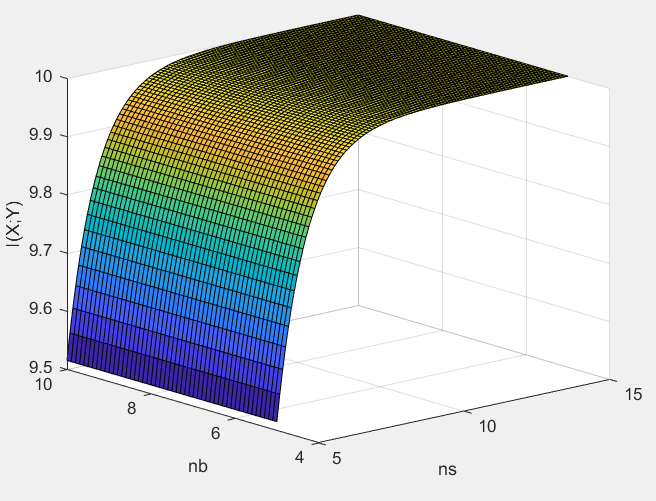
\includegraphics[width=12.5cm]{Image_of_Q2RERE.png}
\end{figure}
\newpage
\subsection{求解OOK调制MIMO互信息}
有$M=2,N=4$,则:$P_r(X_1=0)=P_r(X_1=1)=\frac{1}{2},P_r(X_2=0)=P_r(X_2=1)=\frac{1}{2}$.
\par
记:
\begin{equation*}
    \begin{aligned}
       P(y_n|x_1,x_2)=&P_r(Y=y_n|X_m=x_m,m,1,2) \\
       =&C_N^{y_n}\left[1-exp\left(-\frac{\sum_{m=1}^2h_{m,n}x_{m}n_{sm}+n_b}{N}\right)\right]^{y_n}\left[exp\left(-\frac{\sum_{m=1}^2h_{m,n}x_{m}n_{sm}+n_b}{N}\right)\right]^{N-y_n} \\
       =&P_{n_b}+P_{n_b+h_{1,n}n_{s1}}+P_{n_b+h_{2,n}n_{s2}}+P_{n_b+h_{1,n}n_{s2}}\\
       =&P_0+P_1+P_2+P_{12}
    \end{aligned}
\end{equation*}
其中:
\begin{equation*}
    \begin{aligned}
       P_0&=C_N^{y_n}\left[1-exp\left(-\frac{n_b}{N}\right)\right]^{y_n}\left[exp\left(-\frac{\n_b}{N}\right)\right]^{N-y_n} \\
       P_1&=C_N^{y_n}\left[1-exp\left(-\frac{h_{1,n}n_{s1}+n_b}{N}\right)\right]^{y_n}\left[exp\left(-\frac{h_{1,n}n_{s1}+n_b}{N}\right)\right]^{N-y_n} \\
       P_2&=C_N^{y_n}\left[1-exp\left(-\frac{h_{2,n}n_{s2}+n_b}{N}\right)\right]^{y_n}\left[exp\left(-\frac{h_{2,n}n_{s2}+n_b}{N}\right)\right]^{N-y_n} \\
       P_{12}&=C_N^{y_n}\left[1-exp\left(-\frac{h_{1,n}n_{s1}+h_{2,n}n_{s2}+n_b}{N}\right)\right]^{y_n}\left[exp\left(-\frac{h_{1,n}n_{s1}+h_{2,n}n_{s2}+n_b}{N}\right)\right]^{N-y_n}
    \end{aligned}
\end{equation*}
有:\par
$I(X_1,X_2;Y)=\sum_{n=1}^4I(X_1,X_2;Y_n)$\par
$I(X_1,X_2;Y_n)=H(Y_n)-H(Y_n|X_1,X_2)$
\begin{equation*}
    \begin{aligned}
       H(Y_n)=&-\sum_{y_n=0}^Np(x_1)p(x_2)p(y_n|x_1,x_2)log_2p(x_1)p(x_2)p(y_n|x_1,x_2)\\
       =&-\sum_{y_n=0}^N\frac{1}{4}(P_0+P_1+P_2+P_{12})log_2\left[\frac{1}{4}\left(P_0+P_1+P_2+P_{12}\right)\right] \\
       H(Y_n|X_1,X_2) =& -\sum_{y_n=0}^Np(x_1)p(x_2)\left(P_{0}log_2P_{0}+P_{1}log_2P_{1}+P_{2}log_2P_{2}+P_{12}log_2P_{12}\right) \\
       =& -\sum_{y_n=0}^N\frac{1}{4}(P_{0}log_2P_{0}+P_{1}log_2P_{1}+P_{2}log_2P_{2}+P_{12}log_2P_{12}) \\
       I(X_1,X_2;Y_n)=&H(Y_n)-H(Y_n|X_1,X_2) \\
       =&-\sum_{y_n=0}^N\frac{1}{4}(P_0+P_1+P_2+P_{12})log_2\left[\frac{1}{4}\left(P_0+P_1+P_2+P_{12}\right)\right] \\
       &+\sum_{y_n=0}^N\frac{1}{4}(P_{0}log_2P_{0}+P_{1}log_2P_{1}+P_{2}log_2P_{2}+P_{12}log_2P_{12}) \\
       =&-\sum_{y_n=0}^N\frac{1}{4}(P_0+P_1+P_2+P_{12})log_2\left[\frac{1}{4}\left(\frac{P_0}{P_1}+\frac{P_2}{P_1}+\frac{P_{12}}{P_1}+1\right)\right] \\
       &+ \sum_{y_n=0}^N\frac{1}{4}(P_{0}log_2\frac{P_0}{P_1}+P_{1}log_2\frac{P_2}{P_1}+P_{12}log_2\frac{P_{12}}{P_1}) = I_1+I_2 \\
       I_1=&-\sum_{y_n=0}^N\frac{1}{4}(P_0+P_1+P_2+P_{12})log_2\left[\frac{1}{4}\left(\frac{P_0}{P_1}+\frac{P_2}{P_1}+\frac{P_{12}}{P_1}+1\right)\right] \\
       =& -\sum_{y_n=0}^N\frac{1}{4}(P_0+P_1+P_2+P_{12})log_2\frac{1}{4}\\
       &-\sum_{y_n=0}^N\frac{1}{4}(P_0+P_1+P_2+P_{12})log_2\frac{1}{4}\left(\frac{P_0}{P_1}+\frac{P_2}{P_1}+\frac{P_{12}}{P_1}+1\right)\\
       =& -log_2\frac{1}{4}+I_{11}\\
       I_{11}=&-\sum_{y_n=0}^N\frac{1}{4}(P_0+P_1+P_2+P_{12})log_2\left(\frac{P_0}{P_1}+\frac{P_2}{P_1}+\frac{P_{12}}{P_1}+1\right) \\
       =& -\frac{1}{4}log_2e\sum_{y_n=0}^N(P_0+P_1+P_2+P_{12})ln\left(\frac{P_0}{P_1}+\frac{P_2}{P_1}+\frac{P_{12}}{P_1}+1\right) 
       
    \end{aligned}
\end{equation*}
\begin{equation*}
    \begin{aligned}
       Substituting&\quad ln(x+1)\sim x\quad into\quad I_{11}\quad gives: \\
       I_{11}=& -\frac{1}{4}log_2e\sum_{y_n=0}^N(P_0+P_1+P_2+P_{12})\left(\frac{P_0}{P_1}+\frac{P_2}{P_1}+\frac{P_{12}}{P_1}\right)\\
       =&-\frac{1}{4}log_2e\sum_{y_n=0}^N(P_0+P_2+P_{12})\left(\frac{P_0}{P_1}+\frac{P_2}{P_1}+\frac{P_{12}}{P_1}\right)-\frac{1}{4}log_2e\sum_{y_n=0}^NP_1\left(\frac{P_0}{P_1}+\frac{P_2}{P_1}+\frac{P_{12}}{P_1}\right)\\
       =&\frac{3}{4}log_2e-\frac{1}{4}log_2e\sum_{y_n=0}^N(P_0+P_2+P_{12})\left(\frac{P_0}{P_1}+\frac{P_2}{P_1}+\frac{P_{12}}{P_1}\right)
    \end{aligned}
\end{equation*}
研究任意一个交叉项,记$P_i$中e的指数项为$-\frac{k_i}{N}$:
\begin{equation*}
    \begin{aligned}
       \sum_{y_n=0}^NP_i·\frac{P_j}{P_1}=&\sum_{y_n=0}^NC_N^{y_n}\left(1-e^{-\frac{k_i}{N}}\right)^{y_n}\left(e^{-\frac{k_i}{N}}\right)^{N-y_n}·\frac{C_N^{y_n}\left(1-e^{-\frac{k_j}{N}}\right)^{y_n}\left(e^{-\frac{k_j}{N}}\right)^{N-y_n}}{C_N^{y_n}\left(1-e^{-\frac{k_1}{N}}\right)^{y_n}\left(e^{-\frac{k_1}{N}}\right)^{N-y_n}}\\
        =&\sum_{y_n=0}^NC_N^{y_n}\left[\frac{\left(1-e^{-\frac{k_i}{N}}\right)\left(1-e^{-\frac{k_j}{N}}\right)}{1-e^{-\frac{k_1}{N}}}\right]^{y_n}\left(\frac{e^{-\frac{k_i}{N}}e^{-\frac{k_j}{N}}}{e^{-\frac{k_1}{N}}}\right)^{N-y_n}\\
        I_{11}=&\frac{3}{4}log_2e-\frac{1}{4}log_2e\sum_{i,j=0,2,12}\left[\frac{\left(1-e^{-\frac{k_i}{N}}\right)\left(1-e^{-\frac{k_j}{N}}\right)}{1-e^{-\frac{k_1}{N}}}+\left(\frac{e^{-\frac{k_i}{N}}e^{-\frac{k_j}{N}}}{e^{-\frac{k_1}{N}}}\right)\right]^{N}\\
        I_2=&\sum_{y_n=0}^N\frac{1}{4}(P_{0}log_2\frac{P_0}{P_1}+P_{1}log_2\frac{P_2}{P_1}+P_{12}log_2\frac{P_{12}}{P_1}) = \frac{1}{4}(A+B+C) \\
        A=&\sum_{y_n=0}^NC_N^{y_n}\left(1-e^{-\frac{n_b}{N}}\right)^{y_n}\left(e^{-\frac{n_b}{N}}\right)^{N-y_n}·log_2\left(\frac{1-e^{-\frac{n_b}{N}}}{1-e^{-\frac{n_b+h_{1,n}n_{s1}}{N}}}\right)^{y_n}·\left(e^{-\frac{h_{1,n}n_{s1}}{N}}\right)^{N-y_n} \\ 
        =&\sum_{y_n=0}^NC_N^{y_n}\left(1-e^{-\frac{n_b}{N}}\right)^{y_n}\left(e^{-\frac{n_b}{N}}\right)^{N-y_n}\left[y_n·log_2\left(\frac{1-e^{-\frac{n_b}{N}}}{1-e^{-\frac{n_b+h_{1,n}n_{s1}}{N}}}\right)+\frac{h_{1,n}n_{s1}}{N}(N-y_n)log_2e\right] \\
        =& h_{1,n}n_{s1}·log_2e+N\left(1-e^{-\frac{n_b}{N}}\right)\left[log_2\left(\frac{1-e^{-\frac{n_b}{N}}}{1-e^{-\frac{n_b+h_{1,n}n_{s1}}{N}}}\right)-\frac{h_{1,n}n_{s1}}{N}log_2e\right] \\
        B=&\sum_{y=0}^NP_2log_2\left(\frac{1-e^{-\frac{n_b+h_{2,n}n_{s2}}{N}}}{1-e^{-\frac{n_b+h_{1,n}n_{s1}}{N}}}\right)^{y_n}·\left(e^{-\frac{h_{1,n}n_{s1}-h_{2,n}n_{s2}}{N}}\right)^{N-y_n} \\
        =&(h_{1,n}n_{s1}-h_{2,n}n_{s2})log_2e\\
        &+N\left(1-e^{-\frac{n_b+h_{2,n}n_{s2}}{N}}\right)\left[log_2\left(\frac{1-e^{-\frac{n_b+h_{2,n}n_{s2}}{N}}}{1-e^{-\frac{n_b+h_{1,n}n_{s1}}{N}}}\right)-\frac{h_{1,n}n_{s1}-h_{2,n}n_{s2}}{N}log_2e\right] \\
        C=&-h_{2,n}n_{s2}log_2e+N\left(1-e^{-\frac{n_b+h_{2,n}n_{s2}+h_{1,n}n_{s1}}{N}}\right)\\
        &·\left[log_2\left(\frac{1-e^{-\frac{n_b+h_{2,n}n_{s2}+h_{1,n}n_{s1}}{N}}}{1-e^{-\frac{n_b+h_{2,n}n_{s2}+h_{1,n}n_{s1}}{N}}}\right)-\frac{h_{2,n}n_{s2}}{N}log_2e\right]
    \end{aligned}
\end{equation*}
使用以下代码绘图(具体的代码分析和仿真分析见仿真报告):
\lstinputlisting[
    style       =   Python,
    caption     =   {\bf Matlab Program},
    label       =   {ff.py}
]{Code_of_Q3.txt}
\begin{figure}[htp]
    \centering
    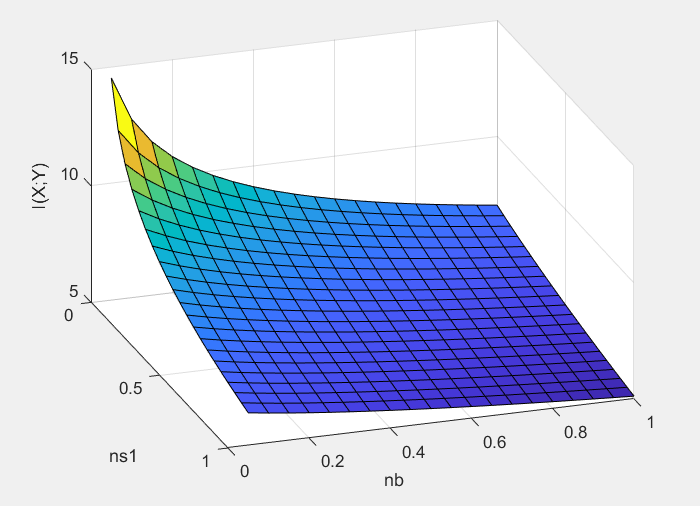
\includegraphics[width=12.5cm]{Image_of_Q3RERE.png}
\end{figure}
\newpage
\subsection{求解大背景光下OOK调制DTP-MIMO互信息}
高斯分布的信息量通式如下:\par
\begin{figure}[htp]
    \centering
    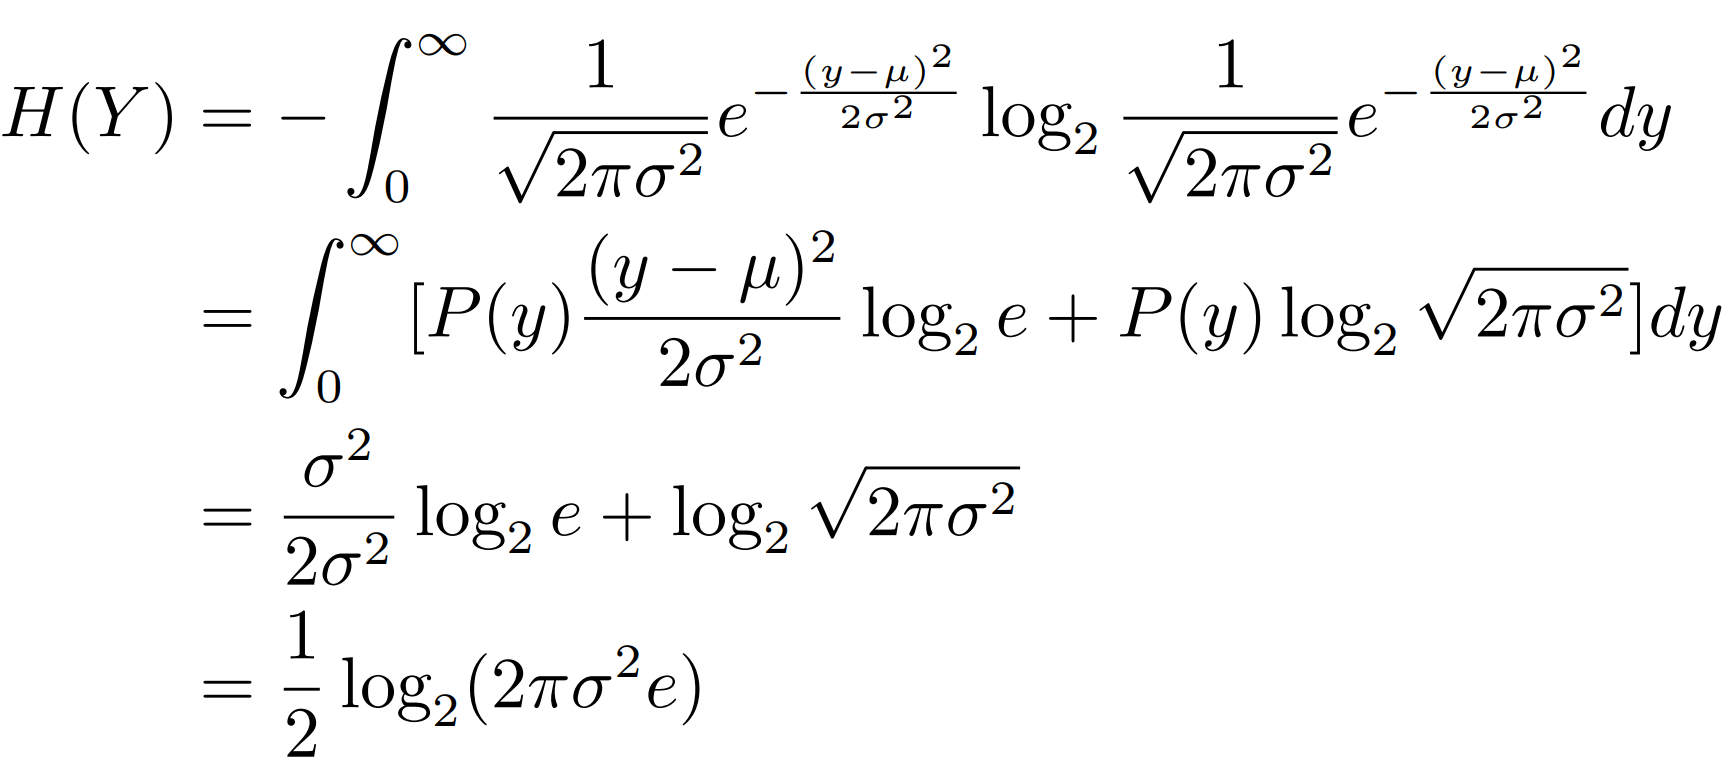
\includegraphics[width=12.5cm]{1.png}
\end{figure}
令$P_1(y)=\frac{1}{\sqrt{2\pi\sigma_1^2}}e^{-\frac{(y-\mu_1)^2}{2\sigma_1^2}}$,$P_2(y)=\frac{1}{\sqrt{2\pi\sigma_2^2}}e^{-\frac{(y-\mu_2)^2}{2\sigma_2^2}}$,则:\par
\begin{figure}[htp]
    \centering
    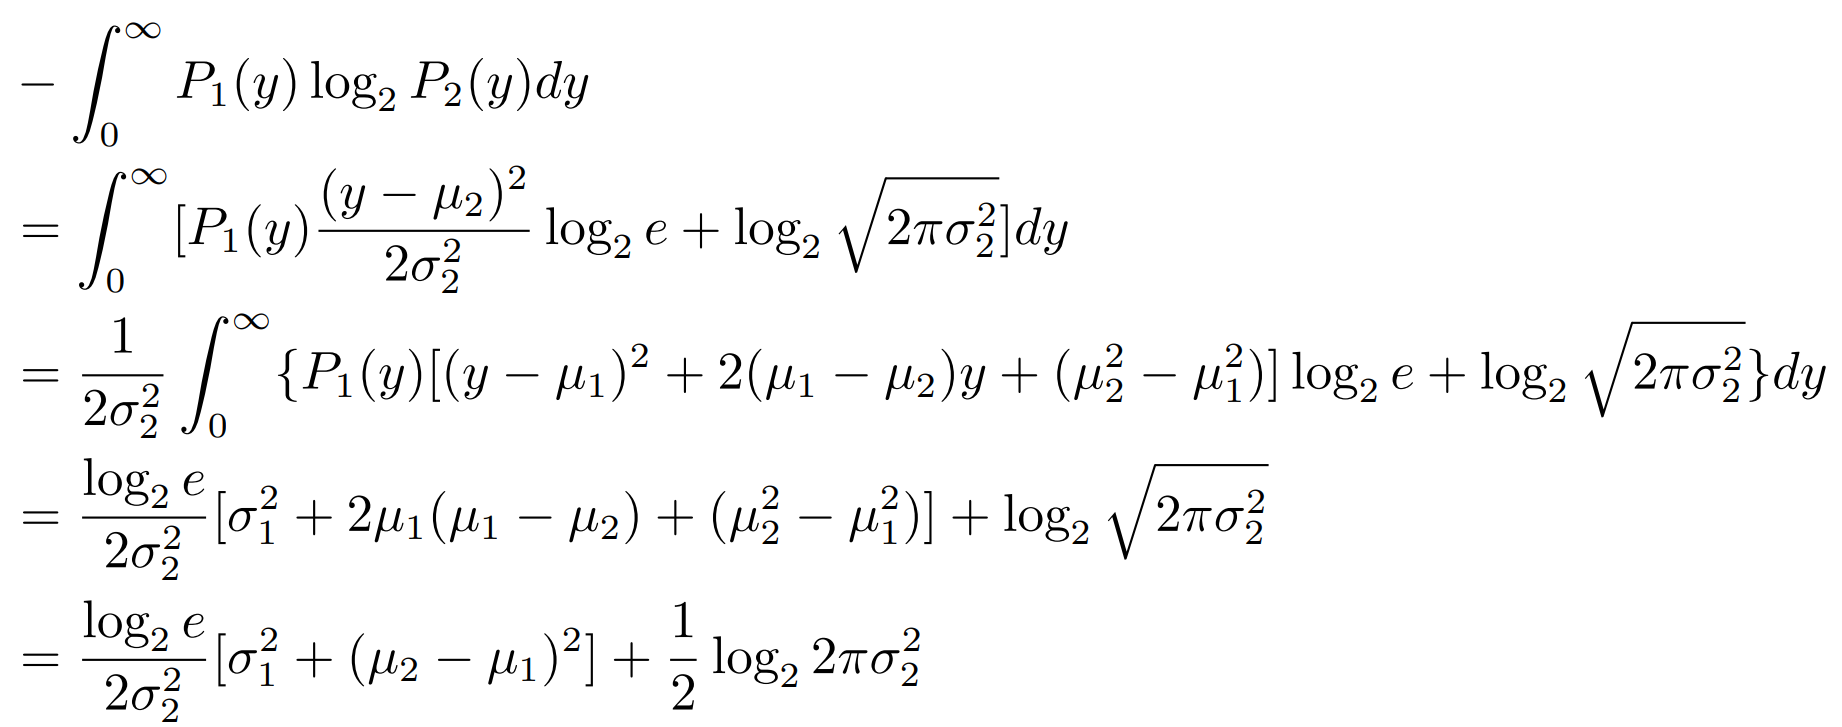
\includegraphics[width=15.8cm]{2.png}
\end{figure}
根据DTP-MIMO的概率密度函数,有:
$$\sigma^2=\mu=\sum_{m=1}^Mh_{m,n}x_mn_{sm}+n_b$$
同时,令:
$$\lambda=\sum_{m=1}^Mh_{m,n}x_mn_{sm}+n_b$$
$$P_1=P_r(Y=y|x_1=0,x_2=0)$$$$P_2=P_r(Y=y|x_1=0,x_2=1)$$$$P_3=P_r(Y=y|x_1=1,x_2=0)$$$$P_4=P_r(Y=y|x_1=1,x_2=1)$$
\newpage
可以得到:\par
\begin{figure}[htp]
    \centering
    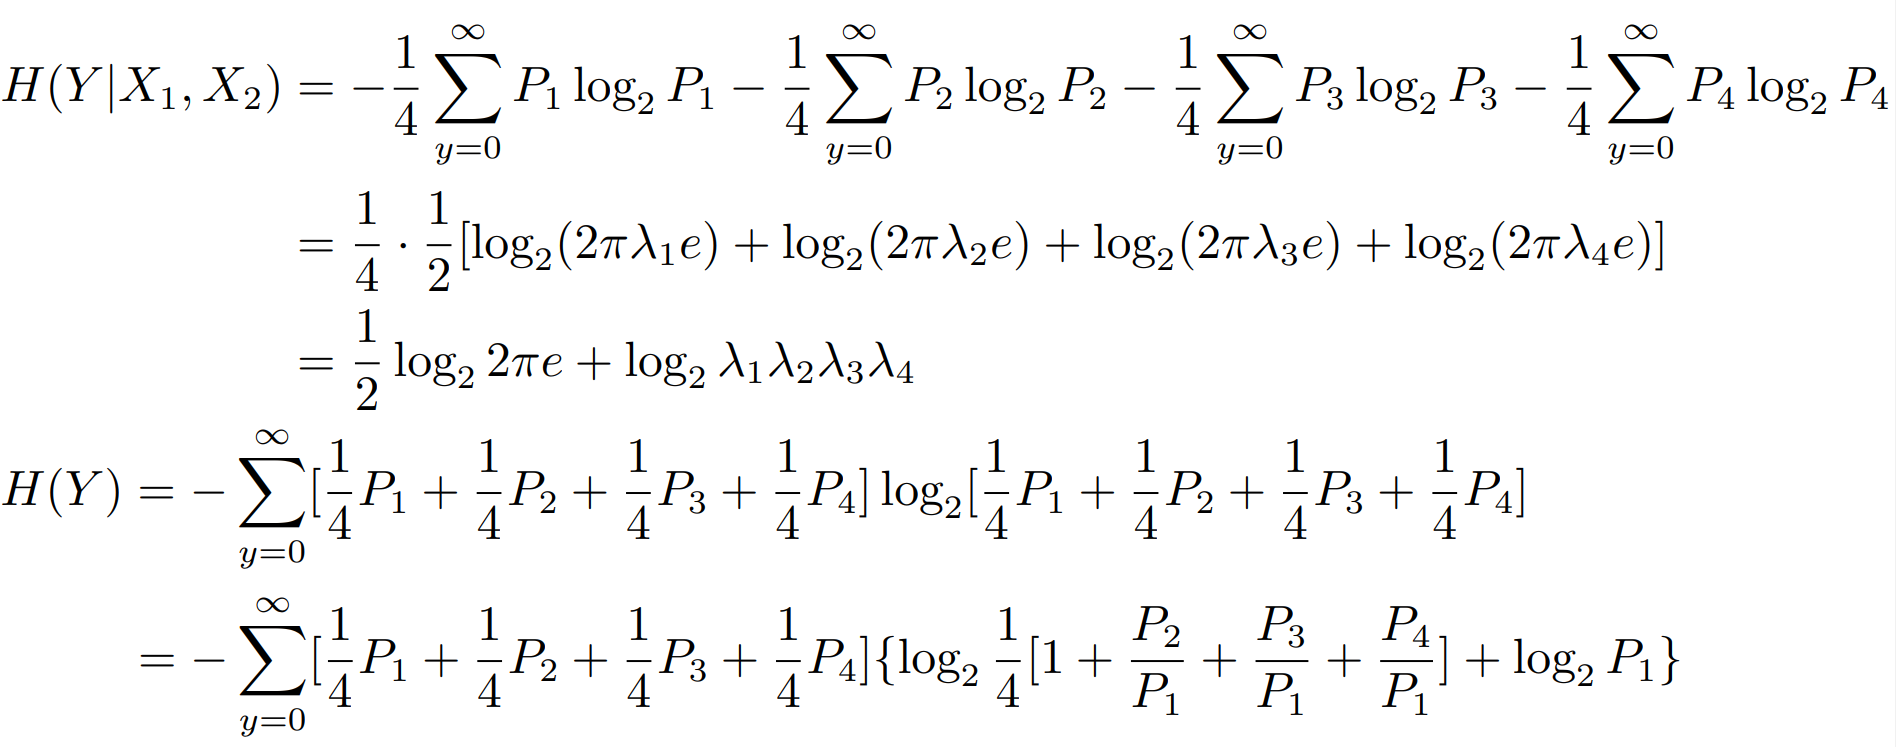
\includegraphics[width=16.9cm]{3.png}
\end{figure}
对$H(Y)$中的加式进行分析可得:\par
\begin{figure}[htp]
    \centering
    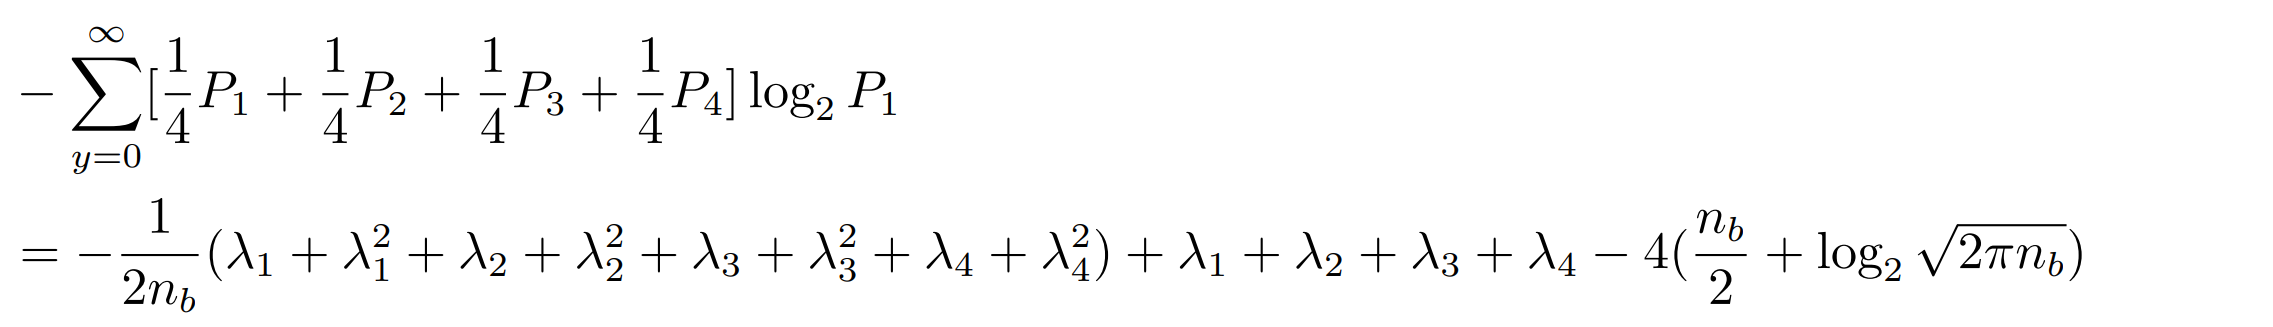
\includegraphics[width=20cm]{4.png}
\end{figure}
对$log$函数进行一阶泰勒展开:\par
\begin{figure}[htp]
    \centering
    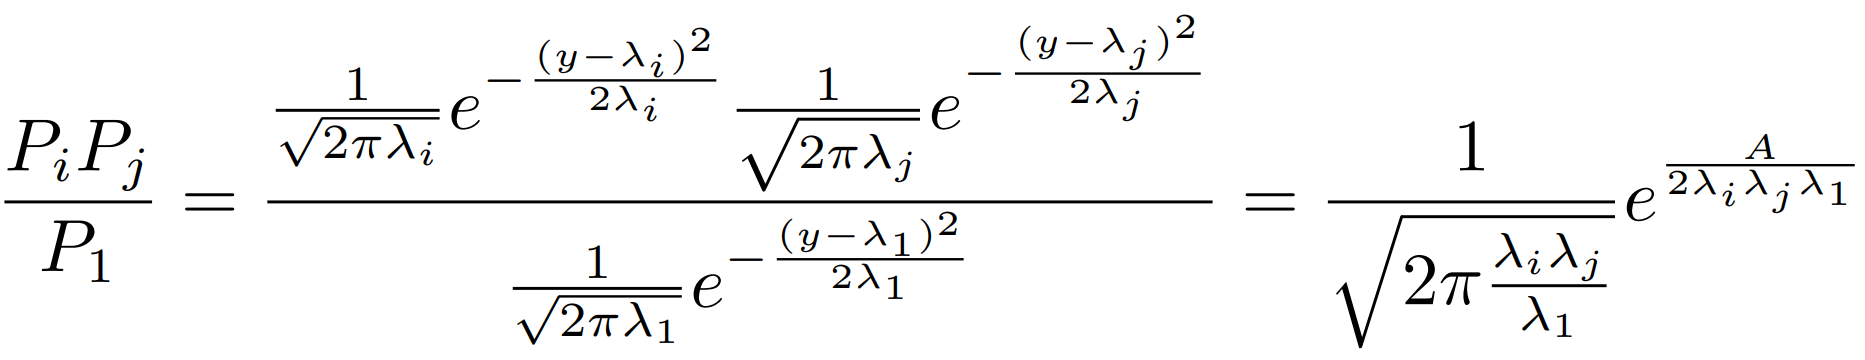
\includegraphics[width=14cm]{5.png}
\end{figure}
\newpage
有:\par
\begin{figure}[htpb]
    \flushleft 
    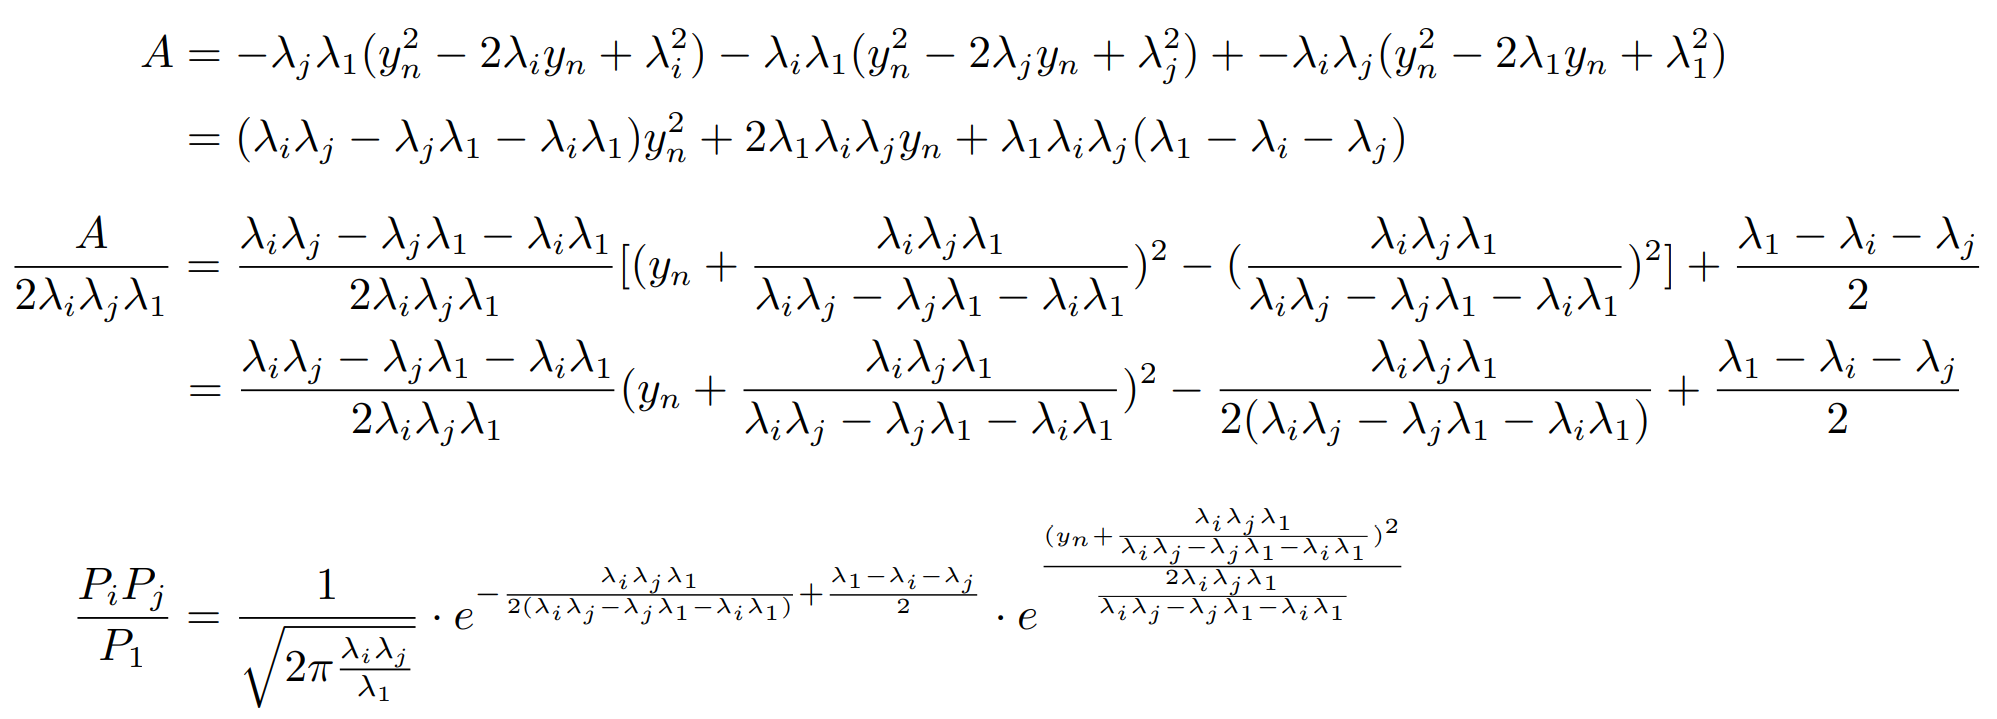
\includegraphics[width=18.8cm]{6.png}
\end{figure}
分析可得,最后一项乘式为$\mu=\sigma^2=\frac{\lambda_i\lambda_j\lambda_1}{\lambda_i\lambda_j-\lambda_i\lambda_1-\lambda_j\lambda_i}$的高斯分布:\par
\begin{figure}[htpb]
    \flushleft 
    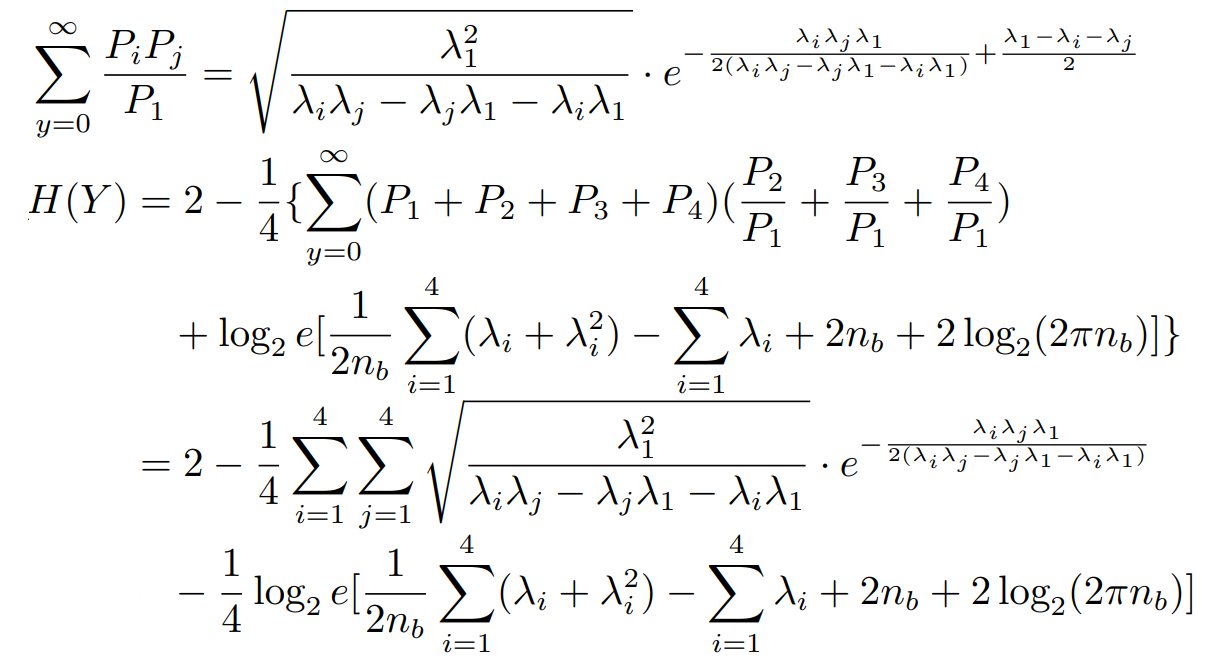
\includegraphics[width=15cm]{7.png}
\end{figure}
\newpage
最后可以得出:\par
\begin{figure}[htpb]
    \flushleft 
    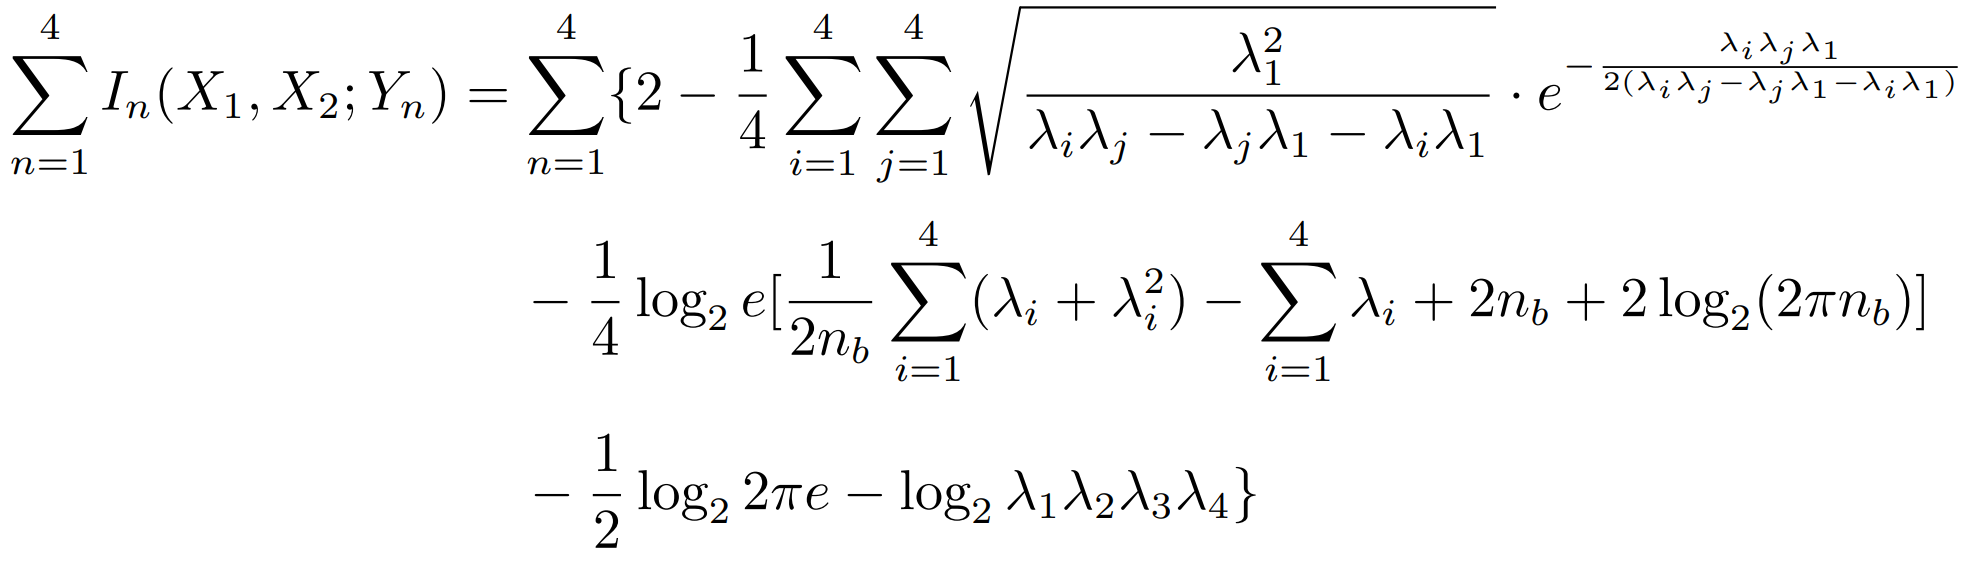
\includegraphics[width=17.1cm]{8.png}
\end{figure}
其中:
\begin{equation*}
    \begin{aligned}
       \lambda_1&=n_b \\
       \lambda_2&=n_b+h_{1,n}n_{s1} \\
       \lambda_3&=n_b+h_{0,n}n_{s0} \\
       \lambda_4&=n_b+h_{1,n}n_{s1}+h_{0,n}n_{s0} 
    \end{aligned}
\end{equation*}
利用$ln(x+1)\approx\frac{m}{2}\left[(x+1)^{\frac{1}{m}}-(x+1)^{-\frac{1}{m}}\right]$有:
\begin{figure}[htpb]
    \flushleft 
    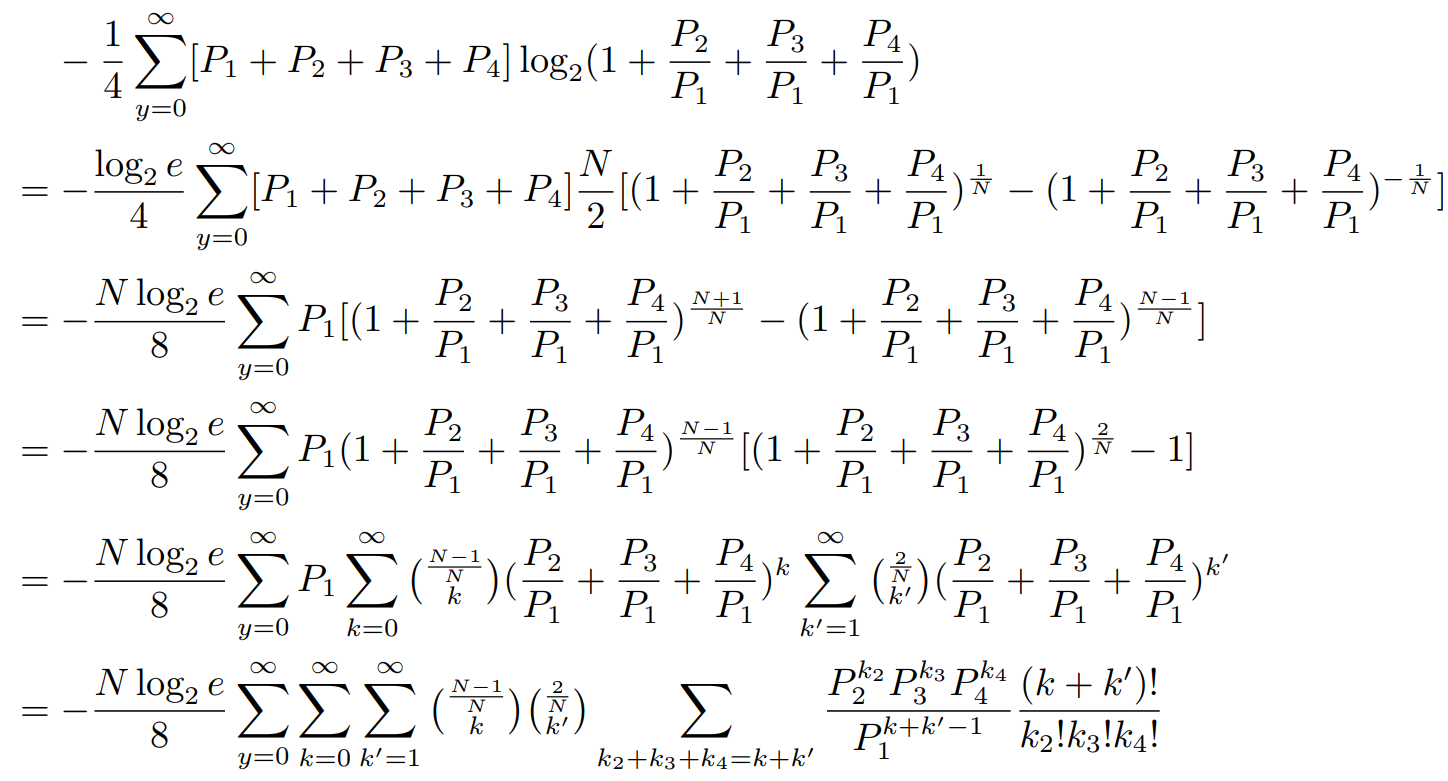
\includegraphics[width=17.1cm]{9.png}
\end{figure}
\newpage
其中:\par
\begin{figure}[htpb]
    \flushleft 
    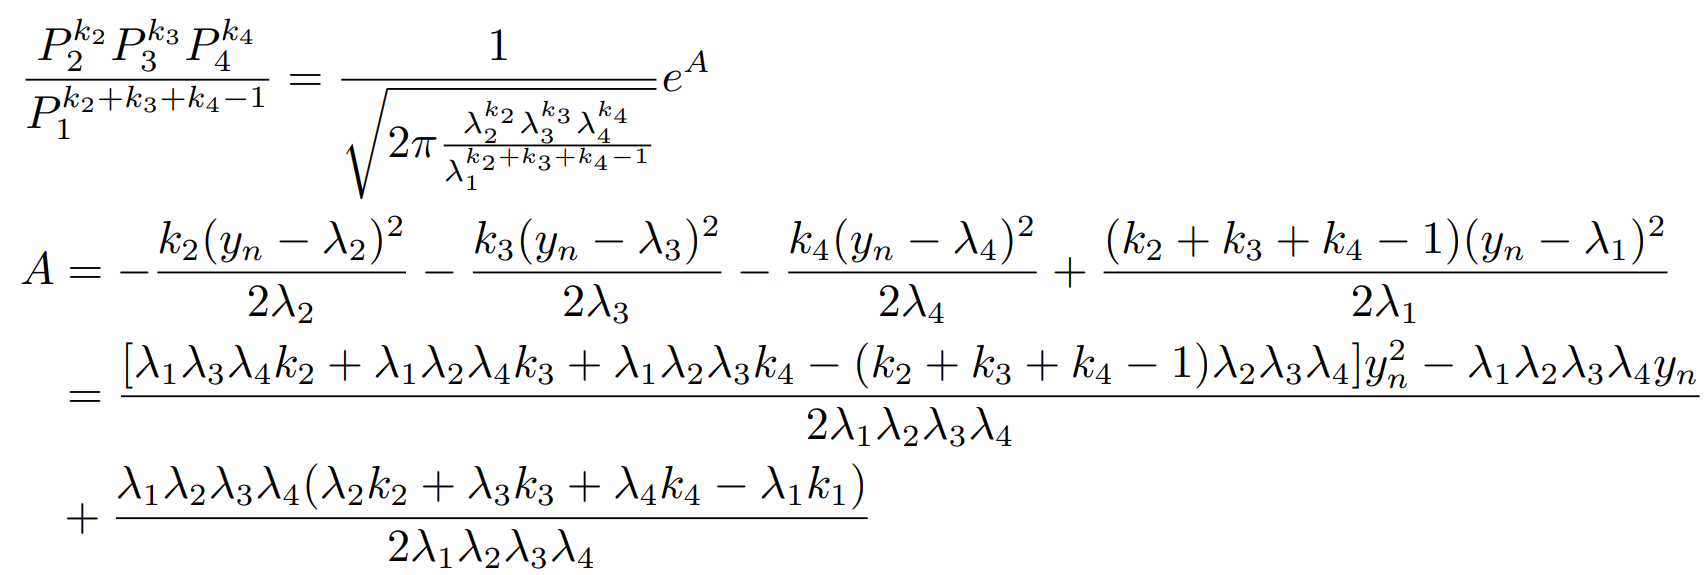
\includegraphics[width=17.4cm]{10.png}
\end{figure}
$e^A$可以看作$\mu=\sigma^2=\frac{\lambda_1\lambda_2\lambda_3\lambda_4}{\lambda_1\lambda_3\lambda_4k_2+\lambda_1\lambda_2\lambda_4k_3+\lambda_1\lambda_2\lambda_3k_4-(k_2+k_3+k_4-1)\lambda_2\lambda_3\lambda_4}$的高斯分布:\par
\begin{figure}[htpb]
    \centering
    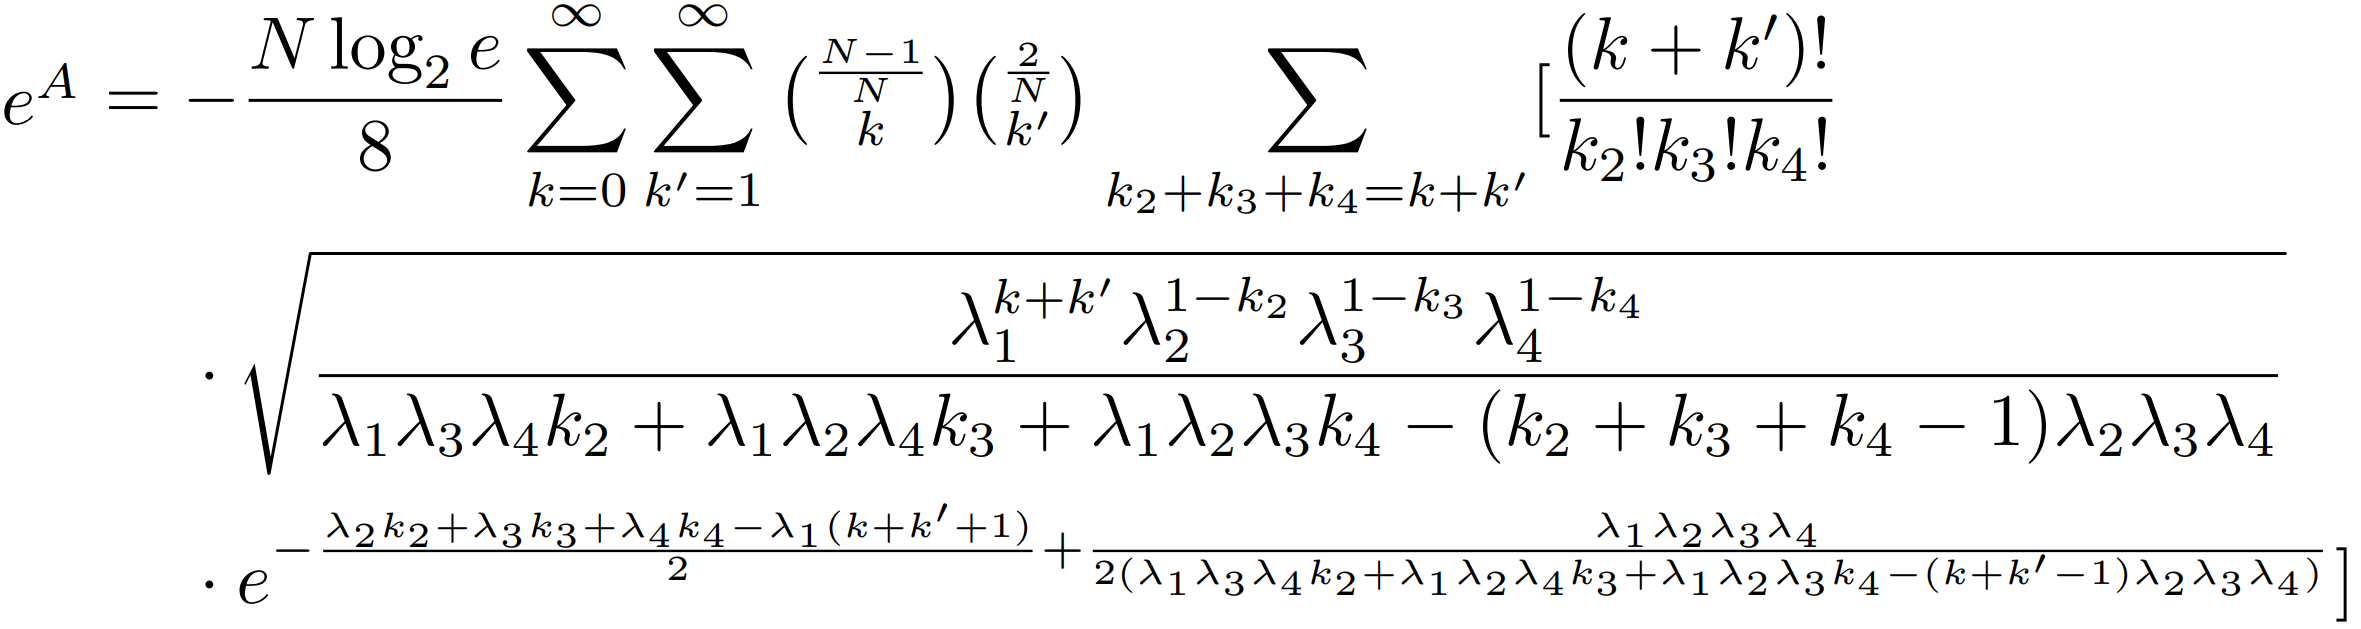
\includegraphics[width=15.4cm]{11.png}
\end{figure}
带回上式:\par
\begin{figure}[htpb]
    \centering
    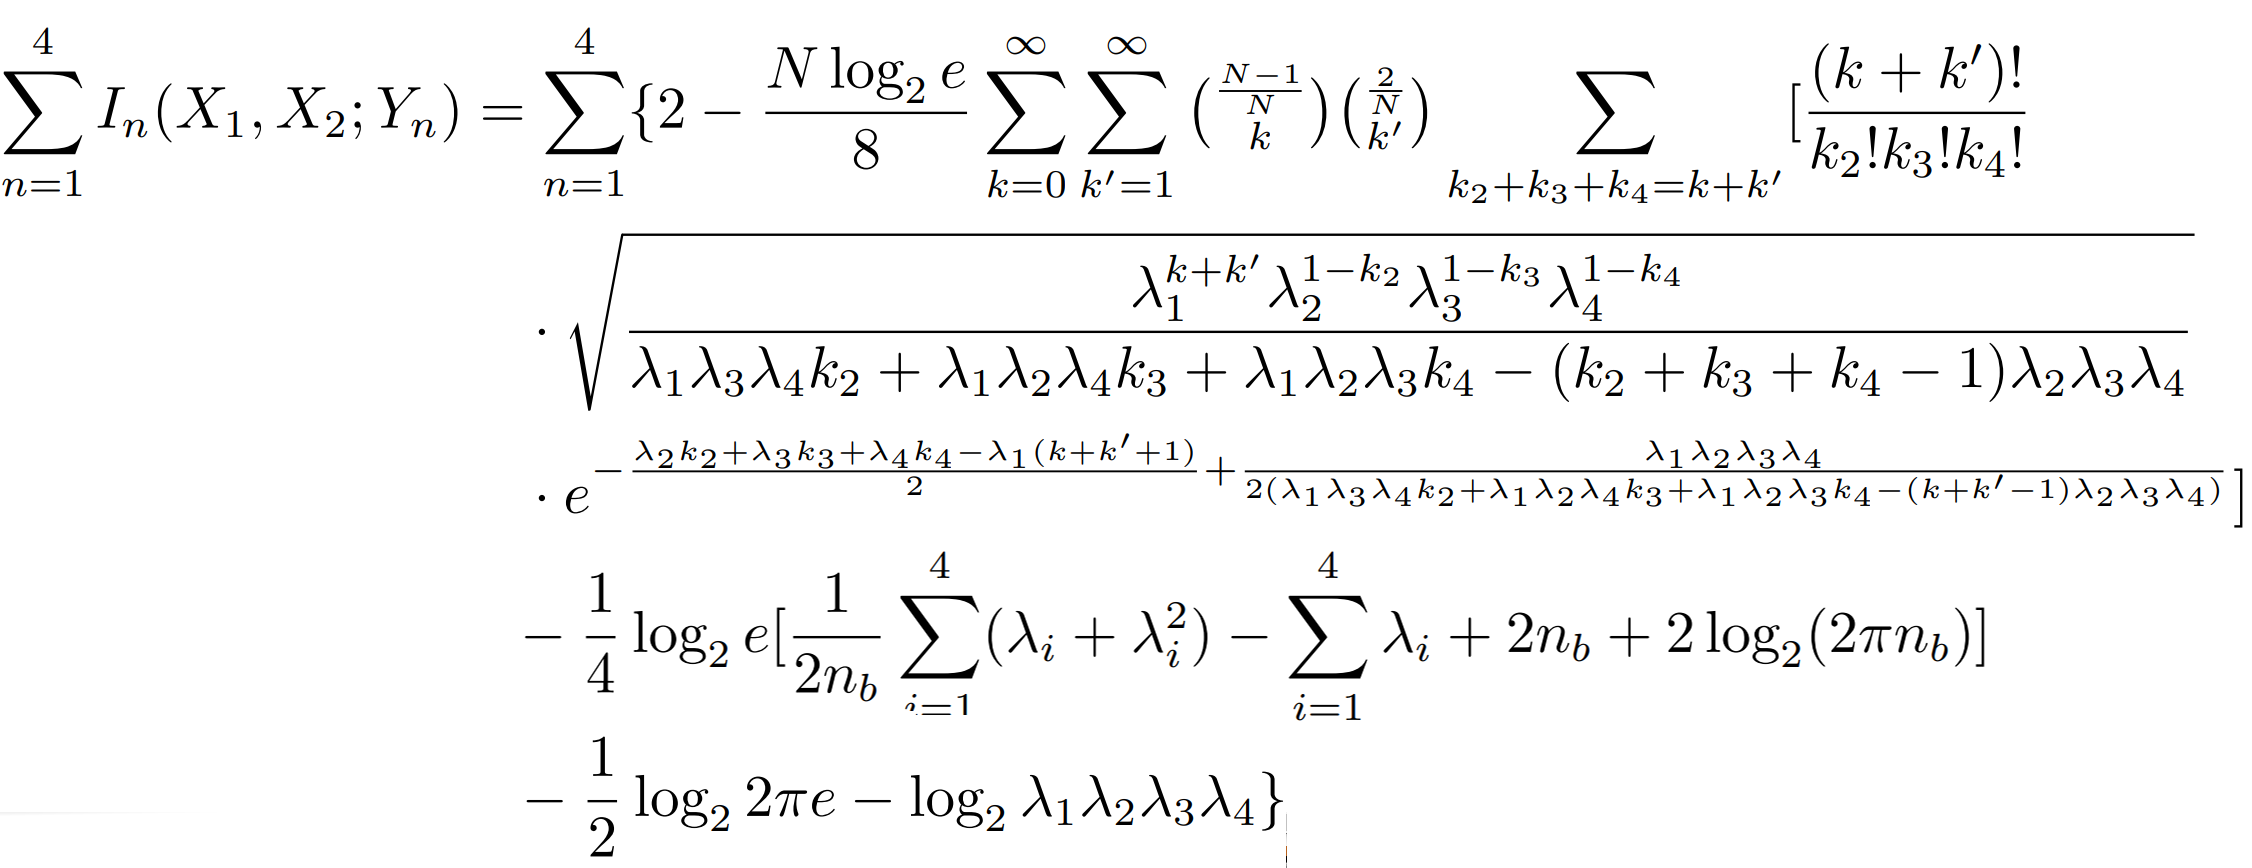
\includegraphics[width=16.5cm]{12.png}
\end{figure}

\newpage
\subsection{求解Q-PAM调制SISO互信息推导至M=M,N=N,Q=Q的情况}
定义$\Lambda_n=Xh_nn_s+n_b,t_i=x_ih_nn_s+n_b,t_Q=n_s+n_b,P_{t_i}(y_n)=Pr(y_n|x_i)=C^{y_n}_{N}\left(1-e^{-\frac{t_i}{N}}\right)^y_n\left(e^{-\frac{t_i}{N}}\right)^{N-y_n}$:
那么有:
\begin{equation*}
  \begin{aligned}
    I(X;Y_n) &= H(Y_n)-H(Y_n|X) \\
      &= -\sum\limits_{j=0}^{N}Pr(y_n_i)log_2Pr(y_n_j)+\sum_{ij}P_{t_i}(y_n_j)P(x_i)log_2P_{t_i}(y_n_j) 
  \end{aligned}
\end{equation*}
$X$的各取值等概,所以$P(x_i)=\frac{1}{Q}$。
\begin{equation*}
  \begin{aligned}
    I(X;Y_n) &= -\sum\limits_{j=0}^{N}\left\{\left[\sum\limits_{i=0}^Q\frac{1}{Q}P_{t_i}(y_n_j)\right]log_2\left[\sum\limits_{i=1}^Q\frac{1}{Q}P_{t_i}(y_n_j)\right]\right\}+\frac{1}{Q}\sum\limits_{j=0}^N\sum\limits_{i=0}^{Q}\left[P_{t_i}(y_n_j)log_2P_{t_i}(y_n_j)\right]  \\
      &= -\frac{1}{Q}\sum\limits_{j=0}^{N}\left\{\left[\sum\limits_{i=0}^QP_{t_i}(y_n_j)\right]log_2\left[\frac{1}{Q}\sum\limits_{i=1}^QP_{t_i}(y_n_j)\right]\right\}+\frac{1}{Q}\sum\limits_{j=0}^N\sum\limits_{i=0}^{Q}\left[P_{t_i}(y_n_j)log_2P_{t_i}(y_n_j)\right]  
      
  \end{aligned}
\end{equation*}
将上式中$\sum\limits_{j=0}^{N}y_n_j$均改为$\sum\limits_{y_n=0}^{N}y_n$后:
\begin{equation*}
  \begin{aligned}
    I(X;Y_n) =& -\frac{1}{Q}\sum\limits_{y_n=0}^{N}\left\{\left[\sum\limits_{i=0}^QP_{t_i}(y_n)\right]\left[log_2\left(\sum\limits_{i=1}^Q\frac{P_{t_i}(y_n)}{P_{t_Q}(y_n)}\right)-log_2Q\right]\right\} \\
    &+ \frac{1}{Q}\sum\limits_{y_n=0}^{N}\left\{\sum\limits_{i=0}^{Q-1}\left[P_{t_i}(y_n)log_2\frac{P_{t_i}(y_n)}{P_{t_Q}(y_n)}\right]\right\} \\
    =& -\frac{1}{Q}\sum\limits_{y_n=0}^{N}\left\{\left[\sum\limits_{i=0}^QP_{t_i}(y_n)\right]\left[log_2\left(\sum\limits_{i=1}^Q\frac{P_{t_i}(y_n)}{P_{t_Q}(y_n)}\right)\right]\right\} + \frac{1}{Q}\left[\sum\limits_{y_n=0}^{N}\sum\limits_{i=0}^{Q-1}P_{t_i}(y_n)\right]·log_2Q \\
    &+ \frac{1}{Q}\sum\limits_{y_n=0}^{N}\left\{\sum\limits_{i=0}^{Q-1}\left[P_{t_i}(y_n)log_2\frac{P_{t_i}(y_n)}{P_{t_Q}(y_n)}\right]\right\} \\
    =& I_1 + log_2Q + I_2
  \end{aligned}
\end{equation*}
$I_1=-\frac{1}{Q}\sum\limits_{y_n=0}^{N}\left\{\left[\sum\limits_{i=1}^QP_{t_i}(y_n)\right]\left[log_2\left(\sum\limits_{i=1}^Q\frac{P_{t_i}(y_n)}{P_{t_Q}(y_n)}\right)\right]\right\}$\par
\par\par 利用Taylor展开:$ln(1+x)\approx x$得到:
$$log_2\left(\sum\limits_{i=1}^Q\frac{P_{t_i}}{P_{t_Q}}\right)=log_2e·ln\left(\sum\limits_{i=1}^{Q-1}\frac{P_{t_i}}{P_{t_Q}}+1\right)\approx log_2e\left(\sum\limits_{i=1}^{Q-1}\frac{P_{t_i}}{P_{t_Q}}\right)$$
\newpage
所以:\par
\begin{equation*}
  \begin{aligned}
    I_1 &= -\frac{1}{Q}log_2e\sum\limits_{y_n=0}^{N}\left[\left(\sum\limits_{i=1}^QP_{t_i}(y_n)\right)\left(\sum\limits_{i=1}^{Q-1}\frac{P_{t_i}(y_n)}{P_{t_Q}(y_n)}\right)\right] \\
    &= -\frac{1}{Q}log_2e\sum\limits_{y_n=0}^{N}\left[\left(\sum\limits_{i=1}^{Q-1}P_{t_i}(y_n)\right)\left(\sum\limits_{i=1}^{Q-1}\frac{P_{t_i}(y_n)}{P_{t_Q}(y_n)}\right)+\sum\limits_{i=1}^{Q-1}P_{t_i}(y_n)\right] \\
    &=  -\frac{1}{Q}log_2e\sum\limits_{y_n=0}^{N}\left[\left(\sum\limits_{i=1}^{Q-1}P_{t_i}(y_n)\right)\left(\sum\limits_{i=1}^{Q-1}\frac{P_{t_i}(y_n)}{P_{t_Q}(y_n)}\right)\right]-\frac{Q-1}{Q}log_2e
  \end{aligned}
\end{equation*}
带入$P_{t_i}(y_n)=Pr(y_n|x_i)=C^{y_n}_{N}\left(1-e^{-\frac{t_i}{N}}\right)^y_n\left(e^{-\frac{t_i}{N}}\right)^{N-y_n}$:\par
\begin{equation*}
    \sum\limits_{y_n=0}^N\left[P_{t_i}(y_n)\frac{P_{t_j(y_n)}}{{P_{t_Q}(y_n)}}\right] =\sum\limits_{y_n=0}^NC_N^y_n\left[\frac{\left(1-e^{-\frac{t_i}{N}}\right)\left(1-e^{-\frac{t_j}{N}}\right)}{1-e^{-\frac{t_Q}{N}}}\right]^y_n·\left(\frac{e^{-\frac{t_i}{N}}·\frac{e^{-\frac{t_j}{N}}}}{e^{-\frac{t_Q}{N}}}\right)^{N-y_n}
\end{equation*}
利用$(a+b)^N=\sum\limits_{y_n=0}^NC_N^y_na^y_nb^{N-y_n}$,并将上一般交叉项代入原$I_1$中,即:\par
\begin{equation*}
  \begin{aligned}
    I_1 &= -\frac{Q-1}{Q}log_2e-\frac{1}{Q}log_2e·\sum_{i,j=1,2,···,Q-1}\left[\frac{\left(1-e^{-\frac{t_i}{N}}\right)\left(1-e^{-\frac{t_j}{N}}\right)}{1-e^{-\frac{t_Q}{N}}}+e^{\frac{t_Q-t_j-t_i}{N}}\right]^N \\
    I_2 &= \frac{1}{Q}\sum\limits_{y_n=0}^N\left\{\sum\limits_{i=0}^{Q-1}\left[P_{t_i}(y_n)log_2\frac{P_{t_i}(y_n)}{P_{t_Q}(y_n)}\right]\right\} \\
    &= \frac{1}{Q}\sum\limits_{y_n=0}^N\left\{\sum\limits_{i=1}^{Q-1}\left[P_{t_i}(y_n)log_2\frac{C_N^y_n\left(1-e^{-\frac{t_i}{N}}\right)^y_n\left(e^{-\frac{t_i}{N}}\right)^{N-y_n}}{C_N^y_n\left(1-e^{-\frac{t_Q}{N}}\right)^y_n\left(e^{-\frac{t_Q}{N}}\right)^{N-y_n}}\right]\right\} \\
    &= \frac{1}{Q}\sum\limits_{y_n=0}^N\left\{\sum\limits_{i=1}^{Q-1}\left[y_nP_{t_i}(y_n)log_2\left(\frac{1-e^{-\frac{t_i}{N}}}{1-e^{-\frac{t_Q}{N}}}\right)+(N-y_n)P_{t_i}(y_n)log_2\left(\frac{e^{-\frac{t_i}{N}}}{e^{-\frac{t_Q}{N}}}\right)\right]\right\}
  \end{aligned}
\end{equation*}
交换求和次序:\par
\begin{equation*}
  \begin{aligned}
    I_2 =& \frac{1}{Q}\sum\limits_{i=1}^{Q-1}\left\{\sum\limits_{y_n=0}^N\left[y_nP_{t_i}(y_n)log_2\left(\frac{1-e^{-\frac{t_i}{N}}}{1-e^{-\frac{t_Q}{N}}}\right)\right] - \sum\limits_{y_n=0}^N\left[y_nP_{t_i}(y_n)log_2\left(\frac{e^{-\frac{t_i}{N}}}{e^{-\frac{t_Q}{N}}}\right)\right]\\ &+N\sum\limits_{y_n=0}^NP_{t_i}(y_n)log_2\left(\frac{e^{-\frac{t_i}{N}}}{e^{-\frac{t_Q}{N}}}\right) \right\}
  \end{aligned}
\end{equation*}
利用$E(y_n)=\sum\limits_{y_n=0}^Ny_nP_{t_i}(y_n)$,二项分布$E(y_n)=N(1-P_i)$,其中$P_i=e^{-\frac{t_i}{N}}$:\par
\begin{equation*}
  \begin{aligned}
    I_2 &= \frac{1}{Q}\sum\limits_{i=1}^{Q-1}\left[N(1-P_i)·log_2\left(\frac{1-e^{-\frac{t_i}{N}}}{1-e^{-\frac{t_Q}{N}}}\right)\right]-\frac{1}{Q}\sum\limits_{i=1}^{Q-1}\left[N(1-P_i)·log_2\left(\frac{e^{-\frac{t_i}{N}}}{e^{-\frac{t_Q}{N}}}\right)\right]+\frac{N}{Q}\sum\limits_{i=1}^{Q-1}log_2\left(\frac{e^{-\frac{t_i}{N}}}{e^{-\frac{t_Q}{N}}}\right)
  \end{aligned}
\end{equation*}
将$I_1,I_2$带入$I(X;Y_n)$:\par
\begin{equation*}
  \begin{aligned}
    I(X;Y_n) &= I_1+I_2+log_2Q,\ let\ e^{-\frac{t_i}{N}}=P_i :\\
    =& log_2Q+\frac{1}{Q}\sum\limits_{i=1}^{Q-1}\left(N(1-P_i)·log_2\frac{1-P_1}{1-P_Q}-N(1-P_i)·log_2\frac{P_1}{P_Q}+Nlog_2\frac{P_i}{P_Q}\right)-\frac{Q-1}{Q}log_2e \\
    &- \frac{1}{Q}log_2e\sum\limits_{i,j=1,2,···,Q-1}\left[\frac{(1-P_i)(1-P_j)}{1-P_Q}+\frac{P_iP_j}{P_Q}\right]^N \\
    =& log_2Q-\frac{Q-1}{Q}log_2e+\frac{N}{Q}\sum\limits_{i=1}^{Q-1}\left[log_2\left(\frac{1-P_i}{1-P_Q}·\frac{P_Q}{P_i}\right)^{1-P_i}·\frac{P_i}{P_Q}\right]\\
    &- \frac{1}{Q}log_2e\sum\limits_{i,j=1,2,···,Q-1}\left[\frac{(1-P_i)(1-P_j)}{1-P_Q}+\frac{P_iP_j}{P_Q}\right]^N
  \end{aligned}
\end{equation*}
以上即为最终结果。
但是,在$ln(1+x)~x$这一步存在一定误差,故我们使用另一个用来直接拟合$lnx$的函数$f(x)=\frac{n}{2}\left(x^{\frac{1}{n}}-x^{-\frac{1}{n}}\right)$,当$n$非常大时,拟合的效果很好。
受限于精力与算力,我们取$n=2$的情况计算,即$lnx~x^{\frac{1}{2}}-x^{-\frac{1}{2}}$,计算如下:
\begin{equation*}
  \begin{aligned}
    I_1 &= -\frac{1}{Q}\sum\limits_{y_n=0}^{N}\left\{\left[\sum\limits_{i=1}^QP_{t_i}(y_n)\right]\left[log_2\left(\sum\limits_{i=1}^Q\frac{P_{t_i}(y_n)}{P_{t_Q}(y_n)}\right)\right]\right\} \\
    &= -\frac{1}{Q}log_2e\sum\limits_{y_n=0}^{N}\left\{\left[\sum\limits_{i=1}^QP_{t_i}(y_n)\right]\left[\left(\sum\limits_{i=1}^Q\frac{P_{t_i}(y_n)}{P_{t_Q}(y_n)}\right)^{\frac{1}{2}}-\left(\sum\limits_{i=1}^Q\frac{P_{t_i}(y_n)}{P_{t_Q}(y_n)}\right)^{-\frac{1}{2}}\right]\right\} \\
    &= -\frac{1}{Q}log_2e\sum\limits_{y_n=0}^{N}\left[P_{t_Q}(y_n)\sum\limits_{i=1}^{Q-1}\frac{P_{t_i}(y_n)}{P_{t_Q}(y_n)}·\left(\sum\limits_{i=1}^{Q-1}\frac{P_{t_i}(y_n)}{P_{t_Q}(y_n)}+1\right)^{\frac{1}{2}}\right]
  \end{aligned}
\end{equation*}
令$a_i=\frac{P_{t_i}}{P_{t_Q}}$带入$I_1$中:
$$I_1=-\frac{1}{Q}log_2e\sum\limits_{y_n=0}^{N}\left[P_{t_Q}(y_n)\sum\limits_{i=1}^{Q-1}a_i·\left(\sum\limits_{i=1}^{Q-1}a_i+1\right)^{\frac{1}{2}}\right]$$
利用无穷级数将$\frac{1}{2}$幂次方展开:
\begin{equation*}
  \begin{aligned}
    I_1 &= -\frac{1}{Q}log_2e\sum\limits_{y_n=0}^{N}\left[P_{t_Q}(y_n)\sum\limits_{i=1}^{Q-1}a_i·\sum\limits_{k=0}^{\infty}\left(^{\frac{1}{2}}_k\right)\left(\sum\limits_{i=1}^{Q-1}a_i\right)^{k}\right] \\
    &= -\frac{1}{Q}log_2e\sum\limits_{y_n=0}^{N}\left[P_{t_Q}(y_n)\sum\limits_{k=0}^{\infty}\left(^{\frac{1}{2}}_k\right)\sum\limits_{k_1+k_2+···+k_{Q-1}=k+1}a_1^{k_1}a_2^{k_2}···a_{Q-1}k_{Q-1}\frac{(k+1)!}{k_1!k_2!···k_{Q-1}!}\right] \\
    =& -\frac{1}{Q}log_2e\sum\limits_{k=0}^{\infty}\left(^{1/2}_k\right)\sum\limits_{\sum_{i=1}^{Q-1}k_i=k+1}\left\{\frac{(k+1)!}{\prod_{i=1}^{Q-1}k_i!}\sum\limits_{y_n=0}^NC_N^y_n\left[\prod_{i=0}^{Q-1}\left(\frac{1-e^{-\frac{t_i}{N}}}{1-e^{-\frac{t_Q}{N}}}\right)^{k_i}·\left(1-e^{-\frac{t_Q}{N}}\right)\right]^y_n\right\} \\
    &·\left[\prod_{i=1}^{Q-1}e^{\left(\frac{(Q-i)n_s}{QN}\right)^{k_i}}e^{-\frac{t_Q}{N}}\right]^{N-y_n}
  \end{aligned}
\end{equation*}
利用二项式定理$\sum_{y_n=0}^NC_N^y_na^y_nb^{N-y_n}=(a+b)^N$带入$I_1$中,令$P_i=e^{\frac{t_i}{N}}$:
$$I_1=-\frac{1}{Q}log_2e\sum\limits_{k=0}^\infty\left(^{1/2}_k\right)\sum\limits_{\sum_{i=1}^{Q-1}k_i=k+1}\left\{\frac{(k+1)!}{\prod_{i=1}^{Q-1}k_i!}\left[(1-P_Q)\prod_{i=1}^{Q-1}\left(\frac{1-P_i}{1-P_Q}\right)^{k_i}+P_Q\prod_{i=1}^{Q-1}e^{\left(\frac{Q-i}{NQ}n_s\right)^{k_i}}\right]^N\right\}$$
$I(X;Y_n)=I_1+I_2+log_2Q$
下面尝试利用n计算$I(X;Y_n)$,即$ln(x)\approx\frac{m}{2}\left(x^{\frac{1}{m}}-x^{-\frac{1}{m}}\right)$:
\begin{equation*}
  \begin{aligned}
    I_1 &= -\frac{1}{Q}\sum\limits_{y_n=0}^N\left\{\left[\sum\limits_{i=1}^QP_{t_i}(y_n)\right]\left[log_2\left(\sum\limits_{i=1}^Q\frac{P_{t_i}(y_n)}{P_{t_Q}(y_n)}\right)\right]\right\} \\
    &=-\frac{m}{2Q}log_2e\sum\limits_{y_n=0}^N\left\{\left[\sum\limits_{i=1}^QP_{t_i}(y_n)\right]\left[\left(\sum\limits_{i=1}^Q\frac{P_{t_i}(y_n)}{P_{t_Q}(y_n)}\right)^{\frac{1}{m}}-\left(\sum\limits_{i=1}^Q\frac{P_{t_i}(y_n)}{P_{t_Q}(y_n)}\right)^{-\frac{1}{m}}\right]\right\} \\
    &=-\frac{m}{2Q}log_2e\sum\limits_{y_n=0}^NP_{t_Q}(y_n)\left[\left(\sum\limits_{i=1}^Q\frac{P_{t_i}(y_n)}{P_{t_Q}(y_n)}\right)^{1+\frac{1}{m}}-\left(\sum\limits_{i=1}^Q\frac{P_{t_i}(y_n)}{P_{t_Q}(y_n)}\right)^{1-\frac{1}{m}}\right]
  \end{aligned}
\end{equation*}
将$a_i=\frac{P_{t_i}(y_n)}{P_{t_Q}(y_n)}$代入:
\begin{equation*}
  \begin{aligned}
    I_1 =& -\frac{m}{2Q}log_2e\sum\limits_{y_n=0}^NP_{t_Q}(y_n)\left\{\sum\limits_{k=0}^\infty\left(^{1+1/m}_k\right)\sum\limits_{k_1+k_2+···+k_{Q-1}=k}a_1^{k_1}···a_{Q-1}^{k_{Q-1}}\frac{k!}{k_1!k_2!···k_{Q-1}!} \\ 
    &-\sum\limits_{g=0}^\infty\left(^{1+1/m}_g\right)\sum\limits_{\sum_{i=1}^{Q-1}g_i=g}a_1^{g_1}···a_{Q-1}^{g_{Q-1}}\frac{g!}{g_1!g_2!···g_{Q-1}!}\right\} \\
    =& -\frac{m}{2Q}log_2e\left\{\sum\limits_{k=0}^\infty\left(^{1+1/m}_k\right)\sum\limits_{\sum_{i=1}^{Q-1}k_i=k}\frac{k!}{\prod_{i=1}^{Q-1}k_i!}\left[\prod_{i=1}^{Q-1}\left(\frac{1-e^{-\frac{t_i}{N}}}{1-e^{-\frac{t_Q}{N}}}\right)^{k_i}·\left(1-e^{-\frac{t_Q}{N}}\right)+\prod_{i=1}^{Q-1}e^{\frac{k_i(t_Q-t_i)-t_Q}{N}}\right]^N \\
    &-\sum\limits_{g=0}^\infty\left(^{1+1/m}_g\right)\sum\limits_{\sum_{i=1}^{Q-1}g_i=g}\frac{g!}{\prod_{i=1}^{Q-1}g_i!}\left[\prod_{i=1}^{Q-1}\left(\frac{1-e^{-\frac{t_i}{N}}}{1-e^{-\frac{t_Q}{N}}}\right)^{g_i}·\left(1-e^{-\frac{t_Q}{N}}\right)+\prod_{i=1}^{Q-1}e^{\frac{g_i(t_Q-t_i)-t_Q}{N}}\right]^N\right\}
  \end{aligned}

\end{equation*}
$I(X;Y)=\sum\limits_{n=1}^zI(X;Y_n)$
由于字母重复,此处把输出信道数量定为$z$。
\subsection{求解大背景光下OOK调制DTP-MIMO互信息推导至M=M,N=N,Q=Q}
将输入信道数量定为$M$,输出信道数量定为$Z$:\par
设:
\begin{equation*}
  \begin{aligned}
    &F=\sum\limits_{m=1}^Mh_{m,n}x_mn_{sm}+n_b\\
    &P(x_m)=\frac{1}{M};X_m=D,m=1,2,3,···,M;D=0,1,···,M-1\\
    &P(y_n|x_1,x_2,···,x_M) = \sum_{x_m=0}^{M-1}C_N^{y_n}\left[1-exp\left(-\frac{\sum_{m=1}^Mh_{m,n}x_mn_{sm}+n_b}{N}\right)\right]^{y_n}\\
    &\left[exp\left(-\frac{\sum_{m=1}^Mh_{m,n}x_mn_{sm}+n_b}{N}\right)\right]^{N-y_n}  = \sum_{x_m=0}^{M-1}P_{x_1x_2···x_M}\\
    & I_n(x_1,x_2,···,x_M;y_n)=H(Y_n)-H(Y_n|x_1,x_2,···,x_M)\\
    & H(Y_n)=-\sum_{y_n=0}^N\frac{1}{M}\left(\sum_{x_m=0}^{M-1}P_{x_1x_2···x_M}\right)log_2\left(\frac{1}{M}\sum_{x_m=0}^{M-1}P_{x_1x_2···x_M}\right)\\
    & H(Y_n|x_1,x_2,···,x_M)=-\sum_{y_n=0}^N\frac{1}{M}\left(\sum_{x_m=0}^{M}P_{x_1x_2···x_M}log_2P_{x_1x_2···x_M}\right) \\
    &I_n(x_1,x_2,···,x_M;Y_n)=-\sum_{y_n=0}^N\frac{1}{M}\left(\sum_{x_M=0}^{M-1}P_{x_1x_2···x_M}\right)log_2\left[\frac{1}{M}\left(\frac{\sum_{x_m=0}^{M}P_{x_1x_2x_3···x_M}}{P_{P_{x_1=x_2=···=x_M=0}}}\right)\right]\\
    &\qquad\qquad\qquad\quad\qquad\qquad\ +\sum_{y_n=0}^{N}\frac{1}{M}\left[\sum_{x_m=0}^M\left(P_{x_1x_2···x_M}log_2\frac{P_{x_1x_2···x_M}}{P_{x_1=x_2=···=x_M=0}}\right)\right]\\
    &\qquad\qquad\qquad\quad\qquad\qquad\ =I_1+I_2\\
    &I_1=-\sum_{y_n=0}^{N}\frac{1}{M}\left(\sum_{x_m=0}^{M}P_{x_1x_2···x_M}\right)log_2\frac{1}{M}-\sum_{y_n=0}^{N}\frac{1}{M}\left(\sum_{x_m=0}^{M}P_{x_1x_2···x_M}\right)log_2\left(\frac{\sum_{x_m=0}^{M}P_{x_1x_2···x_M}}{P_{x_1=x_2=···=x_M=0}}\right)\\
    &\quad=-log_2\frac{1}{M}+I_{11}
  \end{aligned}
\end{equation*}
\newpage
设:
\begin{equation*}
  \begin{aligned}
    &I_{11}=-\frac{1}{M}log_2e\sum_{y_n=0}^{M}\left(\sum_{x_m=0}^{M}P_{x_1x_2···x_M}\right)ln\left(\frac{\sum_{x_M}^MP_{x_1x_2···x_M}}{P_{x_1=x_2=···=x_M=0}}\right)\\
    &\qquad\qquad\qquad=-\frac{1}{M}log_2e\sum_{y_n=0}^{M}\left(\sum_{x_m=0}^{M}P_{x_1x_2···x_M}\right)ln\left(G+1\right)
  \end{aligned}
\end{equation*}
用$ln(x+1)\sim x$代入:
\begin{equation*}
    \begin{aligned}
        &I_{11}=-\frac{1}{M}log_2e\sum_{y_n=0}^{M}\left(\sum_{x_m=0}^{M}P_{x_1x_2···x_M}\right)G\\
        &=-\frac{M^2-1}{M}log_2e-\frac{1}{M}log_2e\sum_{y_n=0}^{N}\left(P_{x_1=x_2=···=0}G\right)G
    \end{aligned}
\end{equation*}
其中:$G=\frac{\left(\sum_{x_m=0}^{M}P_{x_1x_2···x_M}\right)-P_{x_1=x_2=···=x_M=0}}{P_{x_1=x_2=···=0}}$\par
\qquad\ \ $P_{x_1=x_2=···=0}·G=\left(\sum_{x_m=0}^{M}P_{x_1x_2···x_M}\right)-P_{x_1=x_2=···=x_M=0}$\par
研究任意一个交叉项,易知$G·G$展开共有$(M^2-1)^2$项,记为$(M^2-1)^2$种组合,$G·G$展开为两概率相乘,每一个小项中两概率分别为$P_{f_1},P_{f_2}$,其中$P_{f_1}=C_{N}^{y_n}(1-e^{-\frac{F_{f_1}}{N}})^{y_n}·(e^{\frac{F_{f_1}}{N}})^{y_n}$,$f_1,f_2$从$1\sim M^2-1$代表$M^2-1$种结论,$F_{f_1}$代表$F$的第$f_1$种组合。
\begin{equation*}
    \begin{aligned}
        &\sum_{y_n=0}^{N}\frac{P_{f_1}P_{f_2}}{P_{x_1=x_2=···=x_M=0}}=\sum_{y_n=0}^{N}C_{N}^{y}\left[\frac{(1-e^{-\frac{F_{f_1}}{N}})(1-e^{-\frac{F_{f_2}}{N}})}{(1-e^{-\frac{F_{n_b}}{N}})}\right]^{y_n}\left(\frac{e^{-\frac{F_{f_1}}{N}}e^{-\frac{F_{f_2}}{N}}}{e^{-\frac{F_{n_b}}{N}}}\right)^N\\
        &I_1=-log_2\frac{1}{M}-\frac{M^2-1}{M}log_2e-\frac{1}{M}log_2e\sum\limits_{All\ combination\ of\ f_1,f_2}^{(M^2-1)^2}\left[\frac{(1-e^{-\frac{F_{f_1}}{N}})(1-e^{-\frac{F_{f_2}}{N}})}{(1-e^{-\frac{F_{n_b}}{N}})}+\frac{e^{-\frac{F_{f_1}}{N}}e^{-\frac{F_{f_2}}{N}}}{e^{-\frac{F_{n_b}}{N}}}\right]^N\\
        &I_2=\frac{1}{M}\sum_{y_n=0}^{N}\left(\sum_{x_m=0}^{M}P_{x_1x_2···x_M}log_2\frac{P_{x_1···x_M}}{P_{x_1=···=x_M=0}}\right)
    \end{aligned}
\end{equation*}
记每一项为$P_flog_2\frac{P_f}{P_{x_1=···=x_M=0}}$,有$M^2-1$个组合,其中一项为:
\begin{equation*}
    \begin{aligned}
        &\sum_{y_n=0}^{N}P_f·log_2\frac{P_f}{P_{x_1=···=x_M=0}} = \sum_{y_n=0}^{N}C_{N}^{y}(1-e^{-\frac{F_{f}}{N}})^{y_n}(e^{-\frac{F_{f}}{N}})^{N-y_n}·log_2\left(\frac{(1-e^{-\frac{F_{f}}{N}})}{(1-e^{-\frac{F_{n_b}}{N}})}\right)^{y_n}\left(e^{-\frac{n_b-F_f}{N}}\right)^{N-y_n}\\
        &\qquad\qquad\qquad\qquad\qquad\qquad=N(1-e^{-\frac{F_{f}}{N}})\left[log_2\frac{(1-e^{-\frac{F_{f}}{N}})}{(1-e^{-\frac{F_{n_b}}{N}})}-\frac{n_b-F_f}{N}log_2e\right]+(n_b-F_f)log_2e\\
        &I_2=\frac{1}{M}\sum_{f}^{M^2-1}\left\{N(1-e^{-\frac{F_{f}}{N}})\left[log_2\frac{(1-e^{-\frac{F_{f}}{N}})}{(1-e^{-\frac{F_{n_b}}{N}})}-\frac{n_b-F_f}{N}log_2e\right]+(n_b-F_f)log_2e\\\right\}
    \end{aligned}
\end{equation*}


\vfill
\centering\Large{Written By \LaTeX\ and Overleaf Editor}
\end{document}